\documentclass{article}
\usepackage[utf8]{inputenc}
\usepackage[a4paper, total={6in, 8in}]{geometry}
\usepackage{indentfirst}
\usepackage{authblk}
\usepackage{graphicx}
\usepackage{hyperref}

%\usepackage[square,numbers]{natbib}
%\usepackage[square,sort,comma,numbers]{natbib}
\usepackage[style=numeric]{biblatex}
\addbibresource{references.bib}
\usepackage[dvipsnames]{xcolor}

\usepackage{amsmath}
\usepackage{amsthm} % proof environment
\usepackage{amsfonts}
\usepackage{amssymb}
\newtheorem{theorem}{Theorem}%[section]
\newtheorem{corollary}{Corollary}[theorem]
\newtheorem{lemma}[theorem]{Lemma}
\newenvironment{claim}[1]{\par\noindent\underline{Claim:}\space#1}{}
\newenvironment{claimproof}[1]{\par\noindent\underline{Proof:}\space#1}{$\square$}

\usepackage{caption}
\usepackage[shortlabels]{enumitem}
\usepackage{float}
\usepackage{listings}

 % highlighting
 \usepackage{soul}
\definecolor{hlcolor}{HTML}{ffffcc}
\definecolor{hl_gramma_color}{HTML}{ffeeff}
\definecolor{hl_math_typo_color}{HTML}{eeffff}
\sethlcolor{hlcolor}
\DeclareRobustCommand{\hlc}[2]{{\sethlcolor{#1}\hl{#2}}} % highlight using custom color: \hlc{green}{some text}
% \newcommand{\hlg}[1]{\hlc{hl_gramma_color}{#1}}
\newcommand{\hlg}[1]{#1}
\newcommand{\mhl}[1]{\setlength{\fboxsep}{0pt}\colorbox{hlcolor}{$\displaystyle #1$}}
\newcommand{\mhlt}[1]{\setlength{\fboxsep}{0pt}\colorbox{hl_math_typo_color}{$\displaystyle #1$}}

\newcommand{\floor}[1]{\left\lfloor #1 \right\rfloor}
\newcommand{\ceil}[1]{\left\lceil #1 \right\rceil}

%\usepackage{showframe} % for show text borders

\usepackage{tabularx, boldline, makecell} % tables
\usepackage{bm} % for \bm math bold
\usepackage{afterpage} % for special pages geometry

\hypersetup{
  colorlinks=true,
  linkcolor=blue,
  filecolor=blue,
  urlcolor=blue,
  citecolor=OliveGreen
}
\urlstyle{same}
\setlength{\parindent}{2em}
\setlength{\parskip}{1ex}
\captionsetup[figure]{labelfont={bf},name={Fig.},labelsep=period}
\numberwithin{figure}{section}

\title{\huge{\textbf{Zarcanum: A Proof-of-Stake Scheme for Confidential Transactions with Hidden Amounts \hl{(updated, draft)}}}}

\author{\large{sowle}\textsuperscript{1}, \large{koe}\textsuperscript{2}}
\affil{\small{
    \textsuperscript{1}Zano project, \texttt{val@zano.org} \\
    \textsuperscript{2}Independent researcher, \texttt{ukoe@protonmail.com}
}}

\date{\small{March 2022\footnote{Version 4.6. Last update: 2022-03-03. Check \href{https://github.com/hyle-team/docs/tree/master/PoS/PoS_with_HA}{here} for the latest version.}}}


\begin{document}
\maketitle

\begin{abstract}
This article explores a Proof-of-Stake mining algorithm in an environment where amounts are hidden with homomorphic commitments, in particular, using confidential transactions. Our goal was to avoid revealing amounts and other sensitive information (like which output was used to stake a given block) to blockchain observers when doing staking.

Our contribution is a Proof-of-Stake mining scheme that does not reveal amounts and is compatible with ring confidential transactions. Also we present a double-blinded commitments extension for Bulletproofs+ range proof protocol with the corresponding security statements.
\end{abstract}

\section{Notation}
Let $\mathbb{G}$ denote the main subgroup of the Ed25519 curve (\cite{ed25519_site}) and $\mathbb{Z}_p$ denote a ring of integers modulo $p$.

$l$ is the order of $\mathbb{G}$: $l = \#\mathbb{G} = 2^{252} + 27742317777372353535851937790883648493$.

For  any  set $X$, $x \stackrel{\$}{\leftarrow} X$ means uniform  sampling of $x$ at random from $X$. 

For any integers $x$, $y$, $\floor{\frac{x}{y}}$ denotes the integer part of \textit{integer arithmetic} division.


\section{Classic PoS scheme (open amounts)} \label{s_open_amounts}

\indent
In this section we describe how PoS mining was originally implemented in Zano\footnote{This scheme is based on ideas from the PeerCoin project \cite{peercoin_wp}. }.

\indent
Suppose Alice has some unspent outputs and wants to mine a PoS block using one of them as a stake. In such a scenario she acts as follows (Fig. \ref{fig:1.1}):

\begin{enumerate}
\item Gets the hash identifier of the last PoW block in the blockchain, $last\_pow\_id$.

\item Gets the last PoS block in the blockchain and gets the stake kernel hash identifier from it, $last\_pos\_kernel\_id$. Together with $last\_pow\_id$ they are called the ``stake modifier''. It changes each time a new block is added to the blockchain. 

\item Makes set $T$ of all possible timestamps for the new PoS block:
\[ T = \{t : t_{min} \leq t \leq t_{max}, \; t \equiv 0 \mod{15} \} \]
where $t_{min}$ and $t_{max}$ are bound to the current blockchain conditions. For the sake of simplicity we can assume that
\[ t_{min} = \tau - T, \; t_{max} = \tau + T \]
where $T$ is a constant and $\tau$ is the current timestamp established in such a way that it is the same across all the network's nodes.

\item Makes set $U$ of all her unspent transaction outputs (UTXO) that are eligible for staking (i.e.\ not locked, mature enough, etc.). For each output $u$ from $U$ she also precalculates the key image $I_u$.

\item Each pair $(t, u) \in T \times U$ is checked against the PoS winning condition as follows:

    \begin{enumerate}
    \item For output $u$ build \textit{stake kernel} $K_u$ as a concatenation:
    \[ K_u = last\_pow\_id \;\|\; last\_pos\_kernel\_id \;\|\; t \;\|\; I_u \]
    where $I_u$ is the key image of the stake output $u$;
    
    \item Calculate hash $h_u = cn\_fast\_hash(K_u)$\footnote{$cn\_fast\_hash$ is an alias for the Keccak-256 hash function, which is similar to SHA3-256 but differs in padding bits.};
    
    \item Finally, check the main condition:
    \begin{equation} \label{old_pos_main_cond}
    \frac{h_u D}{a_u} \stackrel{?}{\leq} 2^{256} \end{equation} 
    where $D$ is the current PoS difficulty, and $a_u$ is the amount of the stake output $u$.
    
    
    \begin{figure}[ht!]
    \centering
    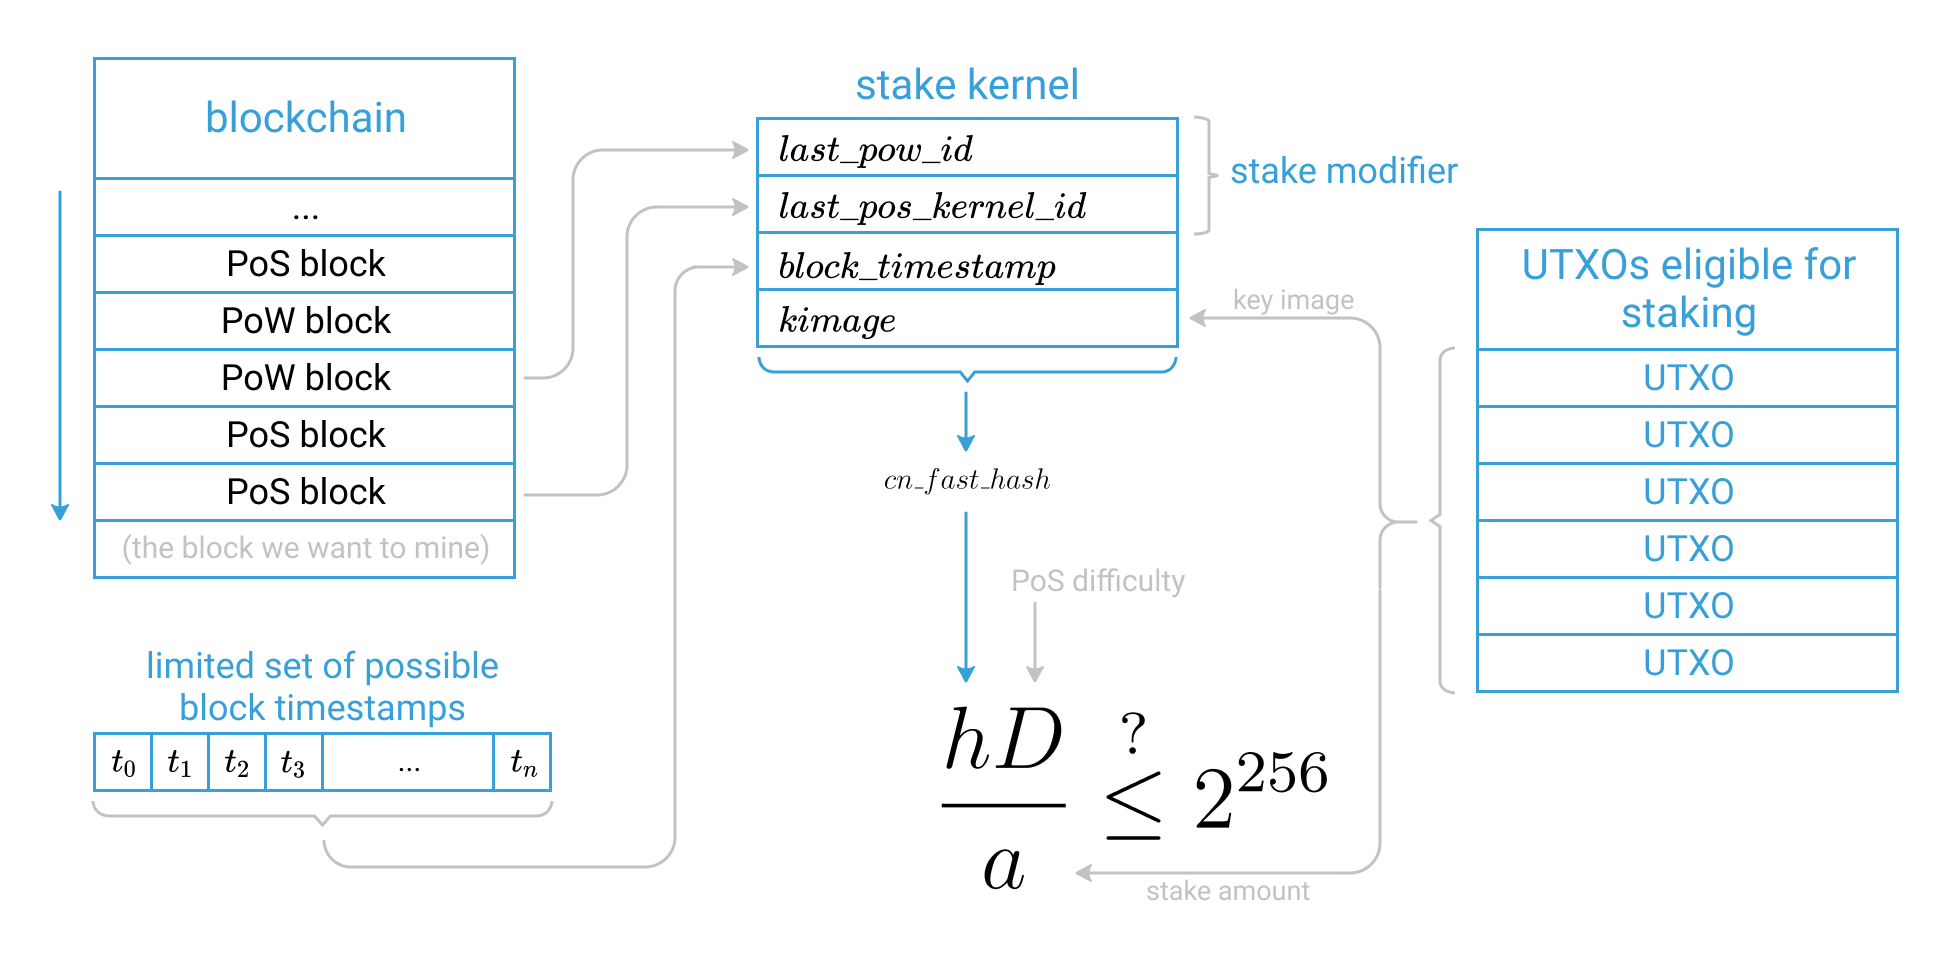
\includegraphics[scale=0.61]{fig_1.png}
    \caption{Scheme of the PoS mining process, as originally implemented in Zano}
    \label{fig:1.1}
    \end{figure}

    \end{enumerate}

    If inequality (\ref{old_pos_main_cond}) holds then it means the success of PoS mining! A block with timestamp $t$ and a stake input spending output $u$ can be constructed and broadcast to the network.
    
\end{enumerate}


If for all pairs $(t, u)$ inequality (\ref{old_pos_main_cond}) does not hold, Alice needs to wait until one of the following happens:
\begin{itemize}
    \item a new block is added to the blockchain (this will change either $last\_pow\_id$\\ or $last\_pos\_kernel\_id$);
    \item some time passes (this will change $t_{min}$ and $t_{max}$).
\end{itemize}

\indent
Once this happens, Alice can attempt mining again (items 1-5), as all $K_u$, and thus $h_u$, will have different values, giving new opportunities to meet the main condition.

We'd like to note the following important property of (\ref{old_pos_main_cond}): as $h_u$ is the result of a cryptographic hash function and can be considered as distributed evenly over the interval $[0, 2^{256})$, the probability of meeting the main condition is proportional to output amount $a_u$. 

%\newpage

\section{Hidden amounts: the problem and the solution} \label{sec_basic_idea}

Consider a hidden amount scheme\footnote{E.g., Confidential Transactions (CT) by Gregory Maxwell \cite{maxwell_ring_ct}.}, where amount $a$ of an output is hidden using Pedersen\footnote{More information in the original paper by T.P.\ Pedersen \cite{Ped}.} commitment $A$:
\[ A = a H + f G \quad (a < 2^{64}, \; f \neq 0) \]
where $H$ and $G$ are generators in $\mathbb{G}$ for which DL relation is unknown, and $f$ is a random hiding mask.

It's easy to see that (\ref{old_pos_main_cond}) can't be used by verifiers anymore because it requires $a$ to be non-hidden. Let's see how the main inequality could be modified.

Suppose Alice has already prepared sets of timestamps ($T$) and outputs ($U$) eligible for staking as mentioned in Section \ref{s_open_amounts}. She then considers each pair $(t, u) \in T \times U$ against the PoS winning condition. She calculates (this time using the hash function $H_s$, which produces scalars in $\mathbb{Z}_l$)\vspace{.115cm}
\[ h = H_s( last\_pow\_id \;\|\; last\_pos\_kernel\_id \;\|\; t \;\|\; I_u ) \]

The use of a hash function means $h$ can be considered as uniform randomness distributed evenly over $\mathbb{Z}_l$. Moreover, since the mask $f$ is $\neq 0$ and fixed for the selected output $u$ (i.e.\ defined before $h$ can be computed), the multiplication $hf \pmod{l}$ can also be considered as uniform randomness over $\mathbb{Z}_l$.

Taking this into account, Alice checks the slightly adjusted PoS winning condition:
\begin{equation} \label{eq_new_ineq_hf}
    hf \bmod{l} \; < \; \floor{\frac{l}{D}}a
\end{equation}
where $l$ is the order of the main subgroup. Here we moved from $2^{256}$ (used originally in (\ref{old_pos_main_cond})) to $l$, as all scalar operations in all the following equations hold modulo $l$ except the division $\floor{\frac{l}{D}}$.

Note that as soon as $D \geq 2^{64}$ and $a < 2^{64}$, the right side of (\ref{eq_new_ineq_hf}) never exceeds $l$.

Now we transform the inequality to equality:
\begin{equation} \label{eq_main_eq}
    hf \; \bmod l \; = \; d a - b_a \;, \quad 1 \leq d \leq \floor{\frac{l}{D}}, \; b_a < 2^{64}
\end{equation}

Once \eqref{eq_new_ineq_hf} holds, Alice needs to calculate $d$ and $b_a$ such that \eqref{eq_main_eq} holds. If she can convince verifiers that she knows $d$ and $b_a$, and that those values are in the correct ranges, she can also convince them that the PoS winning condition \eqref{eq_new_ineq_hf} holds\footnote{Except with negligible probability in the case when $da < b_a$ (see the discussion in Appendix \ref{appendix:brute-force-solution-increase-complexity}, setting $z = 1$).} for a particular $h$, and thus, for a pair $(u, t)$ (assuming she also convinces them that $I_u$ is the key image of an output $u$ that exists in the ledger).

In the following sections we construct such a proof in a NIZK-manner.


\section{Criteria} \label{s_criteria}
Let us make a list of criteria for an ideal PoS mining scheme with hidden amounts to help understand the differences between approaches.

\begin{enumerate}
    \item \textit{(stake proportionality)} The probability of meeting the winning condition is proportional to the stake amount.
    \item \textit{(resistantness)} A miner is unable to tamper with the protocol for their benefit.
    \item \textit{(amount privacy)} Amounts are kept private; hence observers are not able to calculate amounts from public data.
    \item \textit{(sender-recipient anonymity)} The original sender of an output cannot accurately guess when a miner stakes that output and creates a new PoS block.
    \item \textit{(untraceability)} It is unreasonably difficult for observers to determine which output was really used as a stake (e.g.\ when a ring of decoy outputs are used).
\end{enumerate}

It is easy to see that the classic PoS scheme described above in Section \ref{s_open_amounts} satisfies criteria 1, 2 and 5.\footnote{Criterion 5 could be met by using a ring signature to show the key image $I_u$ corresponds to a real output $u$, and also that a pseudo-output commitment corresponds to that output's amount commitment. Then the prover can open the pseudo-commitment to reveal the amount $a_u$, without needing to expose the blinding factor of the original amount commitment (which would break Criterion 5).}

\section{Direct-spend PoS} \label{s_direct_spend_pos_scheme}

In this section, for the sake of clarity, we show how to construct a proof for the winning condition in the simplest case, when there are no decoy outputs, i.e., the stake output is directly referenced in a mining transaction.

Suppose the stake output amount $a$ is committed to in publicly known $A = aH + fG$.

Rewriting \eqref{eq_main_eq} slightly (all scalar equations hold modulo $l$):
\begin{equation} \label{eq_part_a}
    \eqref{eq_main_eq} \quad \Leftrightarrow \quad hf - da + b_a = 0, \quad 1 \leq d \leq \floor{\frac{l}{D}}, \; b_a < 2^{64}
\end{equation}

Let $b_f = df - ha$. The following equality holds:
\begin{equation} \label{eq_part_h}
    ha - df + b_f = 0
\end{equation}

Use \eqref{eq_part_a} and \eqref{eq_part_h} as scalar parts for scalar multiplication with $H$ and $G$ correspondingly:
\begin{equation} \label{eq_ge}
\eqref{eq_part_a}, \eqref{eq_part_h} \Rightarrow
\left\{ \begin{aligned} 
  h f - d a + b_a &= 0 \quad | \times H \\
  h a - d f + b_f &= 0 \quad | \times G
\end{aligned} \right.
\end{equation}

Considering commitments $A'=fH+aG, \; A=aH+fG$, and $B=b_a H + b_f G$, we can rewrite \eqref{eq_ge} in terms of group element operations: 
\begin{equation} 
    hA'-dA+B=\mathbf{0} \label{eq_ge_AA_fin}
\end{equation}
where $\mathbf{0}$ is the identity element of $\mathbb{G}$.

Now to satisfy range requirements in \eqref{eq_main_eq}, Alice needs to reveal $d$ and $A'$, prove that $A'$ is the mirror commitment of $A$, and provide a range proof for $B$ (i.e.\ show that $b_a < 2^{64}$).

Proving the correctness of $A'$ can be done by using mirror commitment proof as shown in Appendix \ref{ss_mirror_commitment_proof}.

This approach satisfies stake proportionality, resistantness, and amount privacy from (\ref{s_criteria}), but the criteria of sender-recipient anonymity and untraceability are not met.

\section{Ring-friendly PoS hidden amount scheme} \label{s_ring_friendly_scheme}

If Alice would like to improve her mining anonymity and use a ring of decoy outputs to hide her stake, she cannot use the approach in Section \ref{s_direct_spend_pos_scheme}, because in a RingCT-like mining transaction with a non-empty decoy set \cite{MRL0005}, the stake input would refer to a \textit{set} of outputs, and thus a \textit{pseudo} output commitment would be used to represent the amount $a$ in the input. Therefore, verifiers on the network would not be able to check \eqref{eq_ge_AA_fin} as they don't know which $A$ from the set of outputs to use.

This problem can be solved if Alice provides another commitment to the same stake amount that verifiers can use in an equation similar to \eqref{eq_ge_AA_fin}, but that can't be used to link to any amount commitment from the ledger.


\subsection{Ring-friendly proof construction}

Let $(V, S) = (vG, sG)$ be Alice's public address, where $v$ and $s$ are her view and spend secret keys correspondingly.

Suppose Alice already went through steps 1-4 in Section \ref{s_open_amounts} and found a pair $(t, u)$ for which the PoS winning condition \eqref{eq_new_ineq_hf} is met. Assume it was Bob who had previously sent output $u$ to Alice. Following the CryptoNote protocol, Bob calculated a one-time address $P$ for output $u$:\footnote{In CryptoNote, a one-time address is calculated as $P_j = H_s(rV, j)G + S$, where $j$ is the index of an output. Here we skip $j$ in $H_s(rV, j)$ for the sake of clarity.}
\[ P = H_s(rV)G + S\] where $r$ is the transaction's secret key. Suppose that for each output Bob also computed group element $Q$ and made it public in addition to $P$:
\[ Q = H_s(rV)V = qG, \; q = vH_s(rV)\]
Note that only Alice and those who get secret view key $v$ from her can calculate secret $q$, as $q = vH_s(vR)$, where $R$ is the transaction's public key.

Recalling equation \eqref{eq_main_eq}, suppose Alice has calculated $d$ and $b_a$ such that the PoS winning equality holds.

Also suppose that, following the standard procedure, she randomly selected a set of apparently unspent decoy outputs $\{u_i\}$ from the blockchain and put her output, which met the PoS main condition \eqref{eq_new_ineq_hf}, at random index $\pi$ of that set.

Let the $i$-th decoy output's commitment be denoted $A_i$ (and $A_\pi$ is the commitment to her own output). Note that in general Alice doesn't know amounts $a_i$ and masks $f_i$ for the outputs she selected as decoys.

Let $X$ be a generator in $\mathbb{G}$ for which the DL relations with $G$ and $H$ are unknown.

Consider extended commitment $C$ to the same stake amount $a$:
\begin{equation} \label{eq_comm_c}
    C = xX + aH + (f + q)G, \quad x \stackrel{\$}{\leftarrow} \mathbb{Z}_l
\end{equation}
Here $x$ is a secret randomness chosen by Alice.

Extended commitment $C$ can be linked to the stake commitment $A_\pi$ (without revealing index $\pi$) by adding two additional layers\footnote{Here we're using terminology and ideas from Multi-layered Linkable Spontaneous Anonymous Group signatures proposed in \cite{MRL0005}.} to the main ring signature:\footnote{If $A_{\pi}$ has a range proof, as it required for confidential transaction amount commitments stored in a ledger, then, taking into account these ring signature layers, observers can be confident that $C$ is composed of the generators $X, H, G$, and that the amount $a$ in $C$ equals the amount $a$ in $A_{\pi}$.}
\begin{enumerate}
    \item a proof of knowing the DL $x$ of $C - A_\pi - Q_\pi$ with respect to $X$;
    \item a proof of knowing the DL $q$ of $Q_\pi$ with respect to $G$.
\end{enumerate}

We can extend the ring signature by adding two group elements to the calculation of the non-interactive challenge as follows:
\begin{equation*} \begin{aligned}
    c_{\pi+1} &= H_s(\dots, \; \alpha_0 X, \; \alpha_1 G) \\
    c_{i+1} &= H_s(\dots, \; r^0_i X + c_i (C - A_{i+1} - Q_{i+1}), \; r^1_i G + c_i Q_{i+1}) \\
    r^0_\pi &= \alpha_0 - c_\pi x \\
    r^1_\pi &= \alpha_1 - c_\pi q \\
 \end{aligned} \end{equation*}

Note that using randomness $x$ in \eqref{eq_comm_c} implies that an external observer would not be able to easily link $C$ with any of $A_i$, even if $a$ and $f$ are known (which is the case for the sender of $A_\pi$).

Consider the mirror extended commitment $C'$:
\begin{equation} \label{eq_comm_c_prime}
    C' = x'X + (f + q)H + aG, \quad x' \stackrel{\$}{\leftarrow} \mathbb{Z}_l, \; x' \neq x
\end{equation}

Let us introduce randomness $x'' \stackrel{\$}{\leftarrow} \mathbb{Z}_l$, $x'' \ne 0$ which is freely chosen by Alice.

Let $b_x = x'' - hx' + dx$. Then the following equation holds:
\begin{equation} \label{eq_part_x}
    hx' - dx + b_x = x''
\end{equation}

Use \eqref{eq_part_a}, \eqref{eq_part_h}, and \eqref{eq_part_x} as scalar parts for scalar multiplication with $H$, $G$, and $X$ correspondingly. Note that we now use $h(f + q)$ instead of $hf$ for \eqref{eq_part_a} and \eqref{eq_part_h}.\footnote{If we do not include $q$ in $h(f + q)$, and instead just have $hf$, then the staked output's sender could check inequality (\ref{eq_main_eq}) for all staking events in the ledger ($d$ and $h$ are public knowledge, and an output's sender knows $f$ and $a$): $da - hf < 2^{64} \pmod l$. The likelihood of that test succeeding yet a different output was staked is negligible, so senders could trivially identify when their outputs are staked by recipients. Including the recipient's secret value $q$ makes that test impossible, preserving sender-recipient anonymity.}
\begin{equation} \label{eq_ge_sys_HGX}
\eqref{eq_part_a}, \eqref{eq_part_h}, \eqref{eq_part_x} \Rightarrow
\left\{ \begin{aligned} 
  h (f + q) - d a + b_a &= 0 \quad &| &\times H \\
  h a - d (f + q) + b_f &= 0 \quad &| &\times G \\
  h x' - d x + b_x &= x'' \quad &| &\times X
\end{aligned} \right.
\end{equation}

Considering $E = b_aH + b_fG + b_xX$ and equations for $C$ and $C'$ above, we can rewrite \eqref{eq_ge_sys_HGX} in terms of group element operations: 
\begin{equation} \label{eq_ge_cc_fin}
    hC'-dC+E=x''X=F
\end{equation}

To convince verifiers that \eqref{eq_ge_cc_fin} holds, Alice discloses $C$, $C'$, and $E$, and provides a Schnorr proof for $F=x''X$. Disclosing $C$, $C'$, and $E$ is safe as each of them are guarded with its own randomness $x$, $x'$, and $x''$ respectively. Alice also needs to prove that $C'$ is in fact the mirror commitment of $C$, and provide a range proof for $E$ to finish proving \eqref{eq_ge_cc_fin}. Proving that \eqref{eq_ge_cc_fin} holds implies that \eqref{eq_part_a} also holds, and thus the PoS winning condition holds as well.


Let us consider these steps in detail.

\begin{enumerate}
    \item Assume the correctness of $C$ is proven by modification of the ring signature (see above).
    
    \item For proving $C' = x'X + (f + q)H + aG$ we use extended mirror commitment proof, described in Appendix \ref{ss_extended_mirror_commitment_proof}.
    
    \item A range proof for $b_a < 2^{64}$ committed to in $E = b_a H + b_f G + b_x X$ can be done directly by extending an existing range proof protocol, like Bulletproofs+\cite{BP+}, to support two blinding factors in commitments. We provide such extension for Bulletproofs+ in Appendix \ref{s_bpp}.
    
    However, this can be achieved using a standard range proof if Alice provides a range proof for commitment $B = b_a H + e G$ on value $b_a$, where $e \stackrel{\$}{\leftarrow} \mathbb{Z}_l$, and also proves that $B$ and $E$ are commitments to the same value $b_a$. The latter can be accomplished by proving that
    \[ E - B = k_0 G + k_1 X\]
    for some $k_0, k_1$ using linear composition proof (\ref{ss_linear_comp_proof}). Indeed: $k_0 = b_f - e$, $k_1 = b_x$.
\end{enumerate}

Note that, if Alice needs to spend her stake output $u$ in the same transaction, which is the case for the PoS protocol used in Zano, she can construct a pseudo output commitment $W = aH + wG$ to the same value $a$ (with $w \stackrel{\$}{\leftarrow} \mathbb{Z}_l$) and provide a linear composition proof for the fact that $C - W = k_0 G + k_1 X$ for some $k_0$ and $k_1$.\footnote{Such a linear composition proof would only show that $W = a H + n_1 G + n_2 X$, where $n_1, n_2 \geq 0$. It is acceptable for $n_2 > 0$ to be true, because any amount balance proof involving $W$ would have to show that $a$ on generator $H$ is canceled out by any new amounts (in the case of a PoS mining transaction, the block reward plus staked output's amount), regardless of statements about values attached to other generators. In practice, setting $n_2 > 0$ may be either impossible (incompatible with balance proofs) or cause new outputs to be unspendable (incompatible with range proofs).}

We believe this approach satisfies all criteria mentioned in Section \ref{s_criteria} above.



\subsection{Ring-friendly scheme outline} \label{ssec_pos_proof}

Let's summarize the whole PoS mining process.

\begin{enumerate}
    \item Alice prepares a set $T$ of possible block timestamps and set $U$ of outputs eligible for staking.
    
    \item For each pair $(t, u)$ she calculates $h = H_s(\dots)$ and $q = vH_s(vR_u)$, and checks the slightly adjusted winning condition \eqref{eq_new_ineq_hf}, using $h(f + q)$ instead of $hf$:
    
    \begin{equation} \label{eq_ineq_hf_plus_q}
    h(f+q) \bmod{l} \; < \; \floor{\frac{l}{D}}a
    \end{equation}
    
    \item If \eqref{eq_ineq_hf_plus_q} holds, she generates random non-zero $x$, $x'$, $x''$ and $e$ in $\mathbb{Z}_l$, and calculates:
    \[ \begin{split}
    d &= \floor{\frac{h(f+q) \bmod l}{a}} + 1\\
    b_a &= da - h(f+q) \\
    b_f &= d(f+q) - ha \\
    b_x &= x'' - hx' + dx \\
    C &= xX + aH + (f+q)G \\
    C' &= x'X + (f+q)H + aG \\
    E &= b_a H + b_f G + b_x X \\
    B &= b_a H + e G
    \end{split}
    \]
    
    \item To prove correctness of $C$ she adds a proof that $C - A_\pi - Q_\pi = xX$ and proof that $Q_\pi = qG$ as additional layers to the main ring signature.
    
    \item To prove correctness of $C'$ she generates two linear composition proofs $(c, y_0, y_1)$, $(c, y_2, y_3)$ for the fact that $C + C' = k_0X + k_1(H+G)$ and $C - C' = k_2X + k_3(H-G)$ (Section \ref{ss_linear_comp_proof}).
    
    \item She generates a Schnorr proof $(c, y_4)$ with respect to base $X$ for the fact that $hC' - dC + E = x''X$.
    
    \item She generates a range proof $\mathcal{R}_B$ showing $b_a < 2^{64}$ in commitment $B$.
    
    \item She generates a linear composition proof $(c, y_5, y_6)$ for the fact that $E - B = k_0G + k_1X$.
    
    \item She makes a PoS block with timestamp $t$, containing a mining transaction with stake output $u$ and extended ring signature, and adds the PoS signature $\sigma$ to the block's data:
    \begin{equation} \label{eq_pos_proof}
        \sigma = \{ d, C, C', E, B, (c, y_0, y_1, y_2, y_3, y_4, y_5, y_6), \mathcal{R}_B \}
    \end{equation}
    Note that all the discrete logarithm proofs can share a Fiat-Shamir challenge $c$.
    
    Also note, that using a range proof protocol with double-blinded commitments (like described in Appendix \ref{s_bpp}) allows to get rid of $B, y_5, y_6$ and makes PoS signature $\sigma$ more compact:
    \[
        \sigma = \{ d, C, C', E, (c, y_0, y_1, y_2, y_3, y_4), \mathcal{R}^e_B \}
    \]
    
\end{enumerate}

\subsection{Verification of ring-friendly PoS scheme} \label{s_verification_ring_friendly}
Verifiers on the network check a PoS block as follows.

\begin{enumerate}
    \item Check $0 < d \leq \floor{\frac{l}{D}}$.
    
    \item Calculate $h = H_s(\dots)$ and $F = hC' - dC + E$.
    
    \item Check the stake input's ring signature, which has additional layers for $C - A_i - Q_i$ and $Q_i$.

    \item Check linear composition proofs $(c, y_0, y_1, y_2, y_3)$ for the fact that $C + C' = k_0X + k_1(H+G)$ and $C - C' = k_2X + k_3(H-G)$.
    
    \item Check Schnorr signature $(c, y_4)$ for the fact that $F = x''X$.
    
    \item Check linear composition proof $(c, y_5, y_6)$ for the fact $E - B = k_0G + k_1X$.

    \item Check range proof $\mathcal{R}_B$.
\end{enumerate}

\subsection{Limitations} \label{s_limitations}

The proposed scheme works only under the following conditions:
\begin{itemize}
    \item Proof-of-stake difficulty: $D > 2^{64}$.
    \item Output's amount: $a < 2^{64}$.
    \item Commitment's mask: $f \neq -q$ (in Appendix \ref{making_sure_f_is_nonzero} we consider this in detail).
\end{itemize}


\subsection{Optional sender-recipient anonymity} \label{ss_no_sender_anonymity_optimization}
If the sender-recipient anonymity criterion mentioned in Section \ref{s_criteria} is considered optional in a particular implementation, the protocol can be simplified as follows:
\begin{itemize}
    \item get rid of $Q$ in outputs' data;
    \item get rid of the additional layer for $Q_\pi = qG$ in the ring signature;
    \item let $q = 0$ in all equations with $q$ above.
\end{itemize}

This data-saving approach can also be used when sender-recipient anonymity is important but it is ensured by other means. For instance, Alice could stake only outputs received from trusted parties (e.g.\ herself), and make other outputs eligible for staking by sending them to herself using a chain of trusted parties.

\subsection{Size of ring-friendly PoS proof}

Let's estimate the size of the proof for $n-1$ decoy outputs, where the total size of the ring is $n$. Assume we're using Bulletproofs+ for range proofing. According to \cite{BP+} it requires $2 \cdot \ceil{\log_2(m) + \log_2(k)} + 3$ elements in $\mathbb{G}$ and 3 elements in $\mathbb{Z}_l$, where $m = 64$ for range $2^{64}$, and $k = 1$ as we only need it for one element $b_a$\footnote{In assumption that the mining transaction or the block has no other suitable Bulletproofs+ that could be aggregated to reduce the size. If there are range proofs that can be aggregated, it is possible to save up to, per additional aggregated proof, 15 elements in $\mathbb{G}$ and 3 elements in $\mathbb{Z}_l$.}.

For the ring signature extension we need to store, presumably, only two extra $\mathbb{Z}_l$ elements per ring member ($r^0_i, r^1_i$).

Additionally, we need to store 9 elements in $\mathbb{Z}_l$ ($d, c, y_0, \dots, y_6$) and 4 elements in $\mathbb{G}$ ($C, C', E, B$) per PoS signature, and one group element per each output in the blockchain ($Q$).

In total we have $19$ group elements and $2n + 12$ field elements. If both field and group elements have a compressed size of 32 bytes, which is the case for Ed25519 used in Zano, then the total size of additional PoS data can be estimated as $2n + 31$ elements per PoS signature and $1$ element per output, or $64n + 992$ bytes per PoS signature and $32$ bytes per output.

If the sender-recipient anonymity is ensured by other means and the protocol is simplified as explained in subsection \ref{ss_no_sender_anonymity_optimization}, the total size of additional data is 19 group elements and $n + 12$ field elements per PoS block. Or, in case of Ed25519, the total size is $n + 31$ elements or $32n + 992$ per PoS block.
%\bibliographystyle{unsrtnat}
%\bibliography{references}
\printbibliography




\newpage
\appendix

\section{Basic proofs}
\subsection{Mirror commitment proof} \label{ss_mirror_commitment_proof}

Suppose Prover ($\mathcal{P}$) needs to convince a Verifier ($\mathcal{V}$) that $A' = fH + aG$ is the mirror commitment of public $A = aH + fG$ without revealing $a$ and $f$. We can construct a Schnorr-like proof as follows.

\begin{theorem}
Let $\mathbb{G}$ be a finite cyclic group where the discrete logarithm problem is hard, and let $\mathbb{F}$ be its scalar field. Let $0 \neq G, H \in \mathbb{G}$ be group elements with no efficiently-computable discrete logarithm relation. We assume that $\mathbb{G}, G, H$ are implicit public parameters where needed. The protocol presented in Fig. \ref{f_mirror_comm_proof_proto} is complete, special sound, and special honest-verifier zero knowledge as a sigma protocol for the relation $\mathcal{R}_1$.
\end{theorem}

\begin{figure}[!ht] % h! -- here
\centering
\begin{tabularx}{0.8\textwidth}
{|>{\hspace{0pt}\vspace{1pt}\raggedright\arraybackslash}X |}
    \hline
    \makecell[c]{\gape{
        %Relation:\\
        $\mathcal{R}_1 = \{ A, A' \in \mathbb{G}; f, a \in \mathbb{F}: A = aH + fG,\  A' = fH + aG\}$
    }} \\
    \hline
    $ \boxed{\mathcal{P}}: r_0, r_1 \stackrel{\$}{\leftarrow} \mathbb{F} $ and computes:\\
    $ \qquad R_0 = r_0 (G + H) $ \\
    $ \qquad R_1 = r_1 (G - H) $ \\
    $\boxed{\mathcal{P} \rightarrow \mathcal{V}}$: $R_0, R_1$ \\
    $\boxed{\mathcal{V}}: c \stackrel{\$}{\leftarrow} \mathbb{F}$ \\
    $\boxed{\mathcal{V} \rightarrow \mathcal{P}}$: $c$ \\
    $\boxed{\mathcal{P}}:$ computes:\\
    $ \qquad y_0 = r_0 + c(a + f) $ \\
    $ \qquad y_1 = r_1 + c(a - f) $ \\
    $\boxed{\mathcal{P} \rightarrow \mathcal{V}}$: $y_0, y_1$ \\
    $\boxed{\mathcal{V}}:$ returns \textit{Accept} if and only if the following hold:
    \begin{align}
        \qquad y_0(H + G) - c(A + A') \stackrel{?}{=} R_0 \label{eq_mirror_comm_proof_v1} \\
        \qquad y_1(H - G) - c(A + A') \stackrel{?}{=} R_1 \label{eq_mirror_comm_proof_v2}
    \end{align} \\
    \hline
\end{tabularx}
\caption{Interactive protocol for mirror commitment proof}
\label{f_mirror_comm_proof_proto}
\end{figure}


\begin{proof}
Completeness follows trivially by inspection.

We next show that the protocol is 2-special sound by a standard rewinding argument, where we define an extractor that produces valid witness elements on accepting transcripts using distinct verifier challenges. Fix an initial transcript $(A, A', R_0, R_1)$, and let $c \neq c'$ be distinct verifier challenges for this transcript, with corresponding responses $(y_0, y_1)$ and $(y'_0, y'_1)$. We apply Equations \eqref{eq_mirror_comm_proof_v1} and \eqref{eq_mirror_comm_proof_v2} to these transcripts to obtain
\[\begin{aligned}
    (y_0 - y'_0) (H + G) - (c - c')(A + A') &= 0 \\
    (y_1 - y'_1) (H - G) - (c - c')(A - A') &= 0 \\
\end{aligned}\]
and hence
\begin{align}
    \frac{y_0 - y'_0}{c - c'} (H + G) = A + A' \label{eq_mirror_comm_poof_v3} \\
    \frac{y_1 - y'_1}{c - c'} (H - G) = A - A' \label{eq_mirror_comm_poof_v4}
\end{align}
Define $\alpha_0 = (y_0 - y'_0) / (c - c')$ and $\alpha_1 = (y_1 - y'_1) / (c - c')$, and note that both are well defined since $c \neq c'$. Adding and subtracting Equations \eqref{eq_mirror_comm_poof_v3} and \eqref{eq_mirror_comm_poof_v4}, we obtain the following expressions for $A$ and $A'$:
\[\begin{aligned}
    A &= \frac{\alpha_0 + \alpha_1}{2} H + \frac{\alpha_0 - \alpha_1}{2} G \\
    A' &= \frac{\alpha_0 - \alpha_1}{2} H + \frac{\alpha_0 + \alpha_1}{2} G
\end{aligned}\]
Hence we define
\[ a = \frac{\alpha_0  + \alpha_1}{2} \]
and
\[ f = \frac{\alpha_0  - \alpha_1}{2} \]
as the extracted witnesses, and the protocol is 2-special sound. Observe that $a$, $f$ must be unique, or this implies a nontrivial discrete logarithm relationship between $G, H$.

We finally show that the protocol is special honest-verifier zero knowledge. To do so, we define a simulator that, on a valid statement and uniformly sampled verifier challenge, produces transcripts indistinguishable from those of real proofs. Fix a valid prover statement $(A, A')$, and sample a nonzero challenge $c \in \mathbb{F}$. The simulator samples random $y_0, y_1 \in \mathbb{F}$ and defines $R_0, R_1$ using Equations \eqref{eq_mirror_comm_proof_v1} and \eqref{eq_mirror_comm_proof_v2}, respectively. The resulting simulated proof will be accepted by an honest verifier. Because $G, H$ are independent generators, such a simulated proof is distributed identically to a real proof, and hence the protocol is special honest-verifier zero knowledge.

This completes the proof.
\end{proof}

This protocol may be made non-interactive via the Fiat-Shamir technique, where the verifier challenge is replaced by a suitable transcript hash. This technique further allows for binding arbitrary proof context into the transcript. In Fig. \ref{f_mirror_comm_proof_ni_proto} such non-interactive protocol is shown as an example.
\begin{figure}[!ht] % h! -- here
\centering
\begin{tabularx}{0.8\textwidth}
{|>{\hspace{0pt}\vspace{1pt}\raggedright\arraybackslash}X |}
    \hline
    \makecell[c]{\gape{
        %Relation:\\
        $\mathcal{R}_1 = \{ A, A' \in \mathbb{G}; f, a \in \mathbb{F}: A = aH + fG,\  A' = fH + aG\}$
    }} \\
    \hline
    $\boxed{\mathcal{P}}: r_0, r_1 \stackrel{\$}{\leftarrow} \mathbb{Z}_l$ and computes:\\
    $ \qquad R_0 = r_0 (H + G),\ R_1 = r_1 (H - G)$ \\
    $ \qquad c = H_s(R_0, R_1, A', A)$ \\
    $ \qquad y_0 = r_0 + c(a+f),\ y_1 = r_1 + c(a-f)$ \\
    $\boxed{\mathcal{P} \rightarrow \mathcal{V}}:(c, y_0, y_1)$ \\
    $\boxed{\mathcal{V}}$: accepts if and only if the following hold: \\
    $ \qquad c \stackrel{?}{=} H_s(y_0(H+G)-c(A+A'),\ y_1(H-G)-c(A-A'),\ A',\ A) $ \\
    \hline
\end{tabularx}
\caption{Non-interactive protocol for mirror commitment proof}
\label{f_mirror_comm_proof_ni_proto}
\end{figure}




\subsection{Extended mirror commitment proof} \label{ss_extended_mirror_commitment_proof}

Suppose a prover ($\mathcal{P}$) needs to convince a verifier ($\mathcal{V}$) that $C' = fH + aG + x'X$ while $C = aH + fG + xX$ is publicly known, $G, H, X \in \mathbb{G}$ are generators without nontrivial DL relations, and scalars $a, f, x, x'$ should not be revealed. For this purpose, we make the following construction.

\begin{theorem}
    Let $\mathbb{G}$ be a finite cyclic group where the discrete logarithm problem is hard, and let $\mathbb{F}$ be its scalar field. Let $0 \neq G, H, X \in \mathbb{G}$ be group elements with no efficiently-computable discrete logarithm relation. We assume that $\mathbb{G}, G, H, X$ are implicit public parameters where needed. The protocol presented in Fig. \ref{f_ex_mirror_comm_proof_proto} is complete, special sound, and special honest-verifier zero knowledge as a sigma protocol for the relation $\mathcal{R}_2$.
\end{theorem}

\begin{figure}[!ht] % h! -- here
\centering
\begin{tabularx}{0.85\textwidth}
{|>{\hspace{0pt}\vspace{1pt}\raggedright\arraybackslash}X |}
    \hline
    \makecell[c]{\gape{
        $\mathcal{R}_2 = \{C,C' \in \mathbb{G};\; f,a,x,x' \in \mathbb{F} : C = aH + fG + xX,\ C' = fH + aG + x'X\} $
    }} \\
    \hline
    $ \boxed{\mathcal{P}}: r_0,r_1,s_0,s_1 \stackrel{\$}{\leftarrow} \mathbb{F} $ and computes:\\
    $ \qquad R_0 = r_0 (H + G) + s_0 X $ \\
    $ \qquad R_1 = r_1 (H - G) + s_1 X $ \\
    $\boxed{\mathcal{P} \rightarrow \mathcal{V}}$: $R_0, R_1$ \\
    $\boxed{\mathcal{V}}: c \stackrel{\$}{\leftarrow} \mathbb{F}$ \\
    $\boxed{\mathcal{V} \rightarrow \mathcal{P}}$: $c$ \\
    $\boxed{\mathcal{P}}$: computes:\\
    $ \qquad y_0 = r_0 + c(a + f) $ \\
    $ \qquad y_1 = r_1 + c(a - f) $ \\
    $ \qquad z_0 = s_0 + c(x + x') $ \\
    $ \qquad z_1 = s_1 + c(x - x') $ \\
    $\boxed{\mathcal{P} \rightarrow \mathcal{V}}$: $y_0, y_1, z_0, z_1$ \\
    $\boxed{\mathcal{V}}:$ returns \textit{Accept} if and only if the following hold:\\
    \begin{align}
        y_0 (H + G) + z_0 X - c(C + C') \stackrel{?}{=} R_0 \label{e_ex_mirror_comm_proof_1} \\
        y_1 (H - G) + z_1 X - c(C - C') \stackrel{?}{=} R_1 \label{e_ex_mirror_comm_proof_2}
    \end{align} \\
    \hline
\end{tabularx}
\caption{Interactive protocol for extended mirror commitment proof}
\label{f_ex_mirror_comm_proof_proto}
\end{figure}


\begin{proof}
    Completeness follows trivially by inspection.

	We next show that the protocol is $2$-special sound by a standard rewinding argument, where we define an extractor that produces valid witness elements on accepting transcripts using distinct verifier challenges.
	Fix an initial transcript $(C,C',R_0,R_1)$, and let $c \neq c'$ be distinct verifier challenges for this transcript, with corresponding responses $(y_0,y_1,z_0,z_1)$ and $(y_0',y_1',z_0',z_1')$.
	We apply Equations \eqref{e_ex_mirror_comm_proof_1} and \eqref{e_ex_mirror_comm_proof_2} to these transcripts to obtain
	\begin{align}
		(y_0 - y_0')(H + G) + (z_0 - z_0')X - (c - c')(C + C') &= 0 \\
		(y_1 - y_1')(H - G) + (z_1 - z_1')X - (c - c')(C - C') &= 0
	\end{align}
	and hence
	\begin{alignat}{1}
		\frac{y_0 - y_0'}{c - c'} (H + G) + \frac{z_0 - z_0'}{c - c'} X &= C + C'	\label{e_ex_mirror_comm_proof_A1_alpha_0} \\	
		\frac{y_1 - y_1'}{c - c'} (H - G) + \frac{z_1 - z_1'}{c - c'} X &= C - C'. \label{e_ex_mirror_comm_proof_A1_alpha_1}
	\end{alignat}
	Define the following:
	\begin{alignat*}{1}
		\alpha_0 &= \frac{y_0 - y_0'}{c - c'} \\
		\alpha_1 &= \frac{y_1 - y_1'}{c - c'} \\
		\beta_0 &= \frac{z_0 - z_0'}{c - c'} \\
		\beta_1 &= \frac{z_1 - z_1'}{c - c'}
	\end{alignat*}
	Note that all are well defined since $c \neq c'$.
	Adding and subtracting Equations \eqref{e_ex_mirror_comm_proof_A1_alpha_0} and \eqref{e_ex_mirror_comm_proof_A1_alpha_1}, we obtain the following expressions for $C$ and $C'$:
	\begin{alignat*}{1}
		C &= \frac{\alpha_0 + \alpha_1}{2} H + \frac{\alpha_0 - \alpha_1}{2} G + \frac{\beta_0 + \beta_1}{2} X \\
		C' &= \frac{\alpha_0 - \alpha_1}{2} H + \frac{\alpha_0 + \alpha_1}{2} G + \frac{\beta_0 - \beta_1}{2} X
	\end{alignat*}
	Hence we define
	\begin{alignat*}{1}
		a &= \frac{\alpha_0 + \alpha_1}{2} \\
		f &= \frac{\alpha_0 - \alpha_1}{2} \\
		x &= \frac{\beta_0 + \beta_1}{2} \\
		x' &= \frac{\beta_0 - \beta_1}{2}
	\end{alignat*}
	as the extracted witnesses, and the protocol is $2$-special sound.
	Observe that $a,f,x,x'$ must be unique, or this implies a nontrivial discrete logarithm relationship between $G,H,X$.

	We finally show that the protocol is special honest-verifier zero knowledge.
	To do so, we define a simulator that, on a valid statement and uniformly-sampled verifier challenge, produces transcripts indistinguishable from those of real proofs.
	Fix a valid prover statement $(C,C')$, and sample a nonzero challenge $c \in \mathbb{F}$.
	The simulator samples random $y_0,y_1,z_0,z_1 \in \mathbb{F}$ and defines $R_0,R_1$ using Equations \eqref{e_ex_mirror_comm_proof_1} and \eqref{e_ex_mirror_comm_proof_2}, respectively.
	The resulting simulated proof will be accepted by an honest verifier.
	Because $G,H,X$ are independent generators, such a simulated proof is distributed identically to a real proof, and hence the protocol is special honest-verifier zero knowledge.

	This completes the proof.
\end{proof}

As above, this protocol may be made non-interactive via the Fiat-Shamir technique, where the verifier challenge is replaced by a suitable transcript hash. In Fig. \ref{f_ex_mirror_comm_proof_ni_proto} such non-interactive protocol is shown as an example.
\begin{figure}[!ht] % h! -- here
\centering
\begin{tabularx}{0.85\textwidth}
{|>{\hspace{0pt}\vspace{1pt}\raggedright\arraybackslash}X |}
    \hline
    \makecell[c]{\gape{
        $\mathcal{R}_2 = \{C,C' \in \mathbb{G};\; f,a,x,x' \in \mathbb{F} : C = aH + fG + xX,\ C' = fH + aG + x'X\} $
    }} \\
    \hline
    $\boxed{\mathcal{P}}: r_0, r_1, s_0, s_1 \stackrel{\$}{\leftarrow} \mathbb{Z}_l$ and computes:\\
    $ \qquad R_0 = r_0 (H + G) + s_0 X,\ R_1 = r_1 (H - G) + s_1 X$ \\
    $ \qquad c = H_s(R_0, R_1, C, C')$ \\
    $ \qquad y_0 = r_0 + c(a+f),\ y_1 = r_1 + c(a-f),\ z_0 = s_0 + c(x+x'),\ z_1 = s_1 + c(x-x')$ \\
    $\boxed{\mathcal{P} \rightarrow \mathcal{V}}:(c, y_0, y_1, z_0, z_1)$ \\
    $\boxed{\mathcal{V}}$: accepts if and only if the following hold: \\
    $ \qquad c \stackrel{?}{=} H_s(y_0(H+G)+z_0X-c(C+C'),\ y_1(H-G)+z_1X-c(C-C'),\ C,\ C') $ \\
    \hline
\end{tabularx}
\caption{Non-interactive protocol for extended mirror commitment proof}
\label{f_ex_mirror_comm_proof_ni_proto}
\end{figure}



\newpage
\subsection{Linear composition proof} \label{ss_linear_comp_proof}

Suppose a prover ($\mathcal{P}$) needs to convince a verifier ($\mathcal{V}$) that $C = aA + bB$, where $A, B \in \mathbb{G}$ are generators without nontrivial DL relations, and scalars $a, b \in \mathbb{Z}_l$ should not be revealed. For this purpose, we can construct a Schnorr-like proof as follows.

\begin{theorem}
    Let $\mathbb{G}$ be a finite cyclic group where the discrete logarithm problem is hard, and let $\mathbb{F}$ be its scalar field. Let $0 \neq A,B \in \mathbb{G}$ be group elements with no efficiently-computable discrete logarithm relation. We assume that $\mathbb{G},A,B$ are implicit public parameters where needed. The protocol presented in Fig. \ref{f_linear_comp_proof_proto} is complete, special sound, and special honest-verifier zero knowledge as a sigma protocol for the relation $\mathcal{R}_3$.
\end{theorem}

\begin{figure}[!ht] % h! -- here
\centering
\begin{tabularx}{0.85\textwidth}
{|>{\hspace{0pt}\vspace{1pt}\raggedright\arraybackslash}X |}
    \hline
    \makecell[c]{\gape{
        $\mathcal{R}_3 = \{C \in \mathbb{G}; a,b \in \mathbb{F} : C = aA + bB\} $
    }} \\
    \hline
    $ \boxed{\mathcal{P}}: r_0,r_1 \stackrel{\$}{\leftarrow} \mathbb{F} $ and computes:\\
    $ \qquad R = r_0 A + r_1 B $ \\
    $\boxed{\mathcal{P} \rightarrow \mathcal{V}}$: $R$ \\
    $\boxed{\mathcal{V}}: c \stackrel{\$}{\leftarrow} \mathbb{F}$ \\
    $\boxed{\mathcal{V} \rightarrow \mathcal{P}}$: $c$ \\
    $\boxed{\mathcal{P}}:$ computes:\\
    $ \qquad y_0 = r_0 + ca $ \\
    $ \qquad y_1 = r_1 + cb $ \\
    $\boxed{\mathcal{P} \rightarrow \mathcal{V}}$: $y_0, y_1$ \\
    $\boxed{\mathcal{V}}:$ returns \textit{Accept} if and only if the following hold:
    \begin{align}
        y_0 A + y_1 B - cC \stackrel{?}{=} R \label{e_linear_comp_proof_check_eq}
    \end{align} \\
    \hline
\end{tabularx}
\caption{Interactive protocol for linear composition proof}
\label{f_linear_comp_proof_proto}
\end{figure}


\begin{proof}
    Completeness follows trivially by inspection.

	We next show that the protocol is $2$-special sound by a standard rewinding argument, where we define an extractor that produces valid witness elements on accepting transcript using distinct verifier challenges.
	Fix an initial transcript $(C,R)$, and let $c \neq c'$ be distinct verifier challenges for this transcript, with corresponding responses $(y_0, y_1)$ and $(y_0', y_1')$.
	We apply Equation \eqref{e_linear_comp_proof_check_eq} to these transcripts to obtain
	$$(y_0 - y_0')A + (y_1 - y_1')B - (c - c')C = 0$$
	and hence
	$$\frac{y_0 - y_0'}{c - c'} A + \frac{y_1 - y_1'}{c - c'} B = C.$$
	Define $$a = \frac{y_0 - y_0'}{c - c'}$$ and $$b = \frac{y_1 - y_1'}{c - c'}$$ as the extracted witnesses, which are well defined since $c \neq c'$, and the protocol is $2$-special sound.
	Observe that $a,b$ must be unique, or this implies a nontrivial discrete logarithm relationship between $A,B$.

	We finally show that the protocol is special honest-verifier zero knowledge.
	To do so, we define a simulator that, on a valid statement and uniformly-sampled verifier challenge, produces transcripts indistinguishable from those of real proofs.
	Fix a valid prover statement $C$, and sample a nonzero challenge $c \in \mathbb{F}$.
	The simulator samples random $y_0,y_1 \in \mathbb{F}$ and defines $R$ using Equation \eqref{e_linear_comp_proof_check_eq},
	The resulting simulated proof will be accepted by an honest verifier.
	Because $A,B$ are independent generators, such a simulated proof is distributed identically to a real proof, and hence the protocol is special honest-verifier zero knowledge.

	This completes the proof.
\end{proof}

This protocol may be made non-interactive via the Fiat-Shamir technique, where the verifier challenge is replaced by a suitable transcript hash. This technique further allows for binding arbitrary proof context into the transcript. In Fig. \ref{f_linear_comp_proof_ni_proto} such non-interactive protocol is shown as an example.
\begin{figure}[!ht] % h! -- here
\centering
\begin{tabularx}{0.8\textwidth}
{|>{\hspace{0pt}\vspace{1pt}\raggedright\arraybackslash}X |}
    \hline
    \makecell[c]{\gape{
        $\mathcal{R}_3 = \{C \in \mathbb{G}; a,b \in \mathbb{F} : C = aA + bB\} $
    }} \\
    \hline
    $\boxed{\mathcal{P}}: r_0, r_1 \stackrel{\$}{\leftarrow} \mathbb{F}$ and computes:\\
    $ \qquad R = r_0 A + r_1 B$ \\
    $ \qquad c = H_s(R, A, B, C)$ \\
    $ \qquad y_0 = r_0 + ca,\ y_1 = r_1 + cb$ \\
    $\boxed{\mathcal{P} \rightarrow \mathcal{V}}:(c, y_0, y_1)$ \\
    $\boxed{\mathcal{V}}$: accepts if and only if the following hold: \\
    $ \qquad c \stackrel{?}{=} H_s(y_0 A + y_1 B - cC,\ A,\ B,\ C) $ \\
    \hline
\end{tabularx}
\caption{Non-interactive protocol for linear composition proof}
\label{f_linear_comp_proof_ni_proto}
\end{figure}





\newpage
\section[How to ensure f != -q]{How to ensure $f \neq -q$} \label{making_sure_f_is_nonzero}

In subsection \ref{s_limitations} we mentioned that the proposed PoS scheme works only under certain conditions, and one of them is the sum $f + q$ must be non-zero for all staking outputs. The reasoning behind that is simple: suppose Alice prepared a UTXO with amount $a$ committed in $A$ with mask $f = -q$: $A = aH - qG$. Such an output can be staked instantly as the winning condition is met regardless of $h$:
\[ hC' - dC + E = x''X \quad \eqref{eq_ge_cc_fin} \quad \stackrel{f = -q}{\Longrightarrow} \quad (b_a - da)H + (b_f + ha)G + (hx'-dx + b_x)X = x''X \]

This implies that for \textit{any} given $h$, Alice can pick arbitrary $b_a < 2^{64}, d, b_f$ such that $b_a = da$ and $b_f = -ha$, and thus all conditions mentioned in subsection \ref{s_verification_ring_friendly} will be satisfied.

Below we show two solutions for this problem: the blockchain-independent method by constructing a special proof and a blockchain-specific method.

\subsection[Proof for f + q != 0]{Proof for $f + q \ne 0$}

Here we construct a proof for $f + q \ne 0$ taking into account criteria from section \ref{s_criteria}. In particular, sender-recipient anonymity must be preserved. We should not allow the sender, who knows $a$ and $f$, to identify the prover.

Consider the following:
\[ C = x X + a H + (f + q) G \]
\[ K = x^{-1} (C - aH) = X + x^{-1}(f + q) G \]
The idea of the proof is to show that $k_0 C + k_1 H = kG + X$ for non-zero $k$.

\noindent
The prover acts as follows:
\begin{enumerate}
    \item Calculates $K = x^{-1} (C - aH)$.
    \item Generates a linear composition proof $(c, y_0, y_1)$ for the fact that $K = k_0 C + k_1 H$ for some $k_0,k_1 \in \mathbb{Z}_l$.
    \item Generates a Schnorr proof $(c, y_2)$ for the fact that $K - X = k G$ for some $k \in \mathbb{Z}_l$.
    Note that $f + q \ne 0$ implies $k \ne 0$.
    \item The proof is $\sigma = \{K, c, y_0, y_1, y_2\}$.
    
    Note that both discrete logarithm proofs can share a Fiat-Shamir challenge $c$.
\end{enumerate}

\noindent
Verifier acts as follows:
\begin{enumerate}
    \item Checks $K \ne X$ (this check ensures that $C$ has a non-zero component of G).
    \item Checks the Schnorr proof $(c, y2)$.
    \item Checks the linear composition proof $(c, y_0, y_1)$.
\end{enumerate}

\noindent
The size of the proof can be estimated as 1 group element and 4 field elements. If both field and group elements have a compressed size of 32 bytes, which is the case for Ed25519 used in Zano, then the total size of additional data is 5 elements, or 160 bytes. Note that the Fiat-Shamir challenge can be shared with other discrete logarithm proofs.


\subsection{Blockchain-specific solution}

Let's require adding $f'H$ and $f'G$ to commitments $C$ and $C'$ respectively before using them in the PoS protocol, where $f'$ is a non-zero public constant that is unknown to a sender when he generates hiding mask $f$ for the output (so he has no way to define $f$ such that $f + q + f' = 0$).

In the case of the Zano blockchain, which has a hybrid PoW/PoS consensus\footnote{More info in the Zano whitepaper \cite{zano_wp}.}, $f'$ can be calculated as $f' = H_s(last\_pow\_id)$, where $last\_pow\_id$ is the hash identifier of the last PoW block in the blockchain\footnote{This would also require that the real output and all the decoy outputs in the staking ring signature to be either older than, or the same age as, the most recent PoW block. Verifiers on the network can easily check such a requirement. Note that  $last\_pow\_id$ is also used as part of the $stake\_modifier$ as described in Section~\ref{s_open_amounts}.}. That way, a malicious miner would have no chance to choose $f$ for his benefit by building an alternative PoS subchain.

Consequently, substituting $f+q+f'$ for $f+q$ in \eqref{eq_new_ineq_hf} we get this modified PoS winning condition:
\begin{equation*}
    h(f+q+f') \bmod{l} \; < \; \floor{\frac{l}{D}}a
\end{equation*}

Doing the same for \eqref{eq_ge_sys_HGX} we get:
\begin{equation*}
\left\{ \begin{aligned} 
  h (f + q + f') - d a + b_a &= 0 \quad &|& \times H \\
  h a - d (f + q + f') + b_f &= 0 \quad &|& \times G \\
  h x' - d x + b_x &= x'' \quad &|& \times X
\end{aligned} \right.
\end{equation*}

Now for \eqref{eq_ge_cc_fin} we obtain:
\[ hC' - dC + E + f'(hH - dG) = x''X \]

With such a modification, neither Alice nor the staked output's sender will be able to gain an advantage when choosing $f$.




\newpage
\section{Brute-force attack, its complexity, and mitigation}
The weak point of the scheme proposed in Section \ref{s_ring_friendly_scheme} is the relation between public scalars $d$ and $h$, sender-known scalars $a$ and $f$, and secret scalar $q$:
\[
d = \floor{\frac{h(f+q) \bmod l}{a}} + 1
\]
An adversarial sender can reveal secret $q$ by guessing $k \in [0; a-1]$ as follows:
\[
q = h^{-1}((d - 1)a + k) - f 
\]
And then reveal Alice's secret view key: $v = (H_s(rV))^{-1}q$, where $r$ is the transaction's secret key which is known to the sender.

\subsection{Complexity}
An adversarial sender would need to scan the blockchain and for each PoS block that is referencing his output in the miner transaction, guess $k$ and check $Q_j \stackrel{?}{=} qG$ for each attempt. The most expensive operation here is EC scalar multiplication, and each attempt would require one such operation. The average number of attempts when testing an output that was staked is upper-bounded at $\frac{1}{2}a$.

Let us use the Zano blockchain as a reference for estimation. As the vast majority of PoS blocks in Zano now have their stake value in $[100 \cdot 10^{12}; 600 \cdot 10^{15}]$, the expected number of attempts can be roughly estimated as $2^{50}$ in practice, which arguably isn't secure enough given that the reward is Alice's secret view key $v$.  

Below we suggest two ways of mitigation: by increasing the complexity of the attack and by eliminating all risk to secret $v$.

\subsection{Solution 1: increasing complexity}
\label{appendix:brute-force-solution-increase-complexity}

We start with a modification of the direct-spend scheme (Section \ref{s_direct_spend_pos_scheme}). Let $z = const$. Consider the following modification to \eqref{eq_part_a} and \eqref{eq_ge_AA_fin}:
\begin{equation} \label{eq_ge_AA_fin_with_z}
    hf - dza + b_a = 0, \quad 1 \leq d \leq \floor{\frac{l}{zD}}, \; b_a < z2^{64}
\end{equation}
\[
    hA' - dzA + B = \mathbf{0}
\]

As the range of $b_a$ is $z$ times bigger, it would require the range proof for $B$ to be extended correspondingly.

For the ring-friendly scheme variant, equation \eqref{eq_ge_cc_fin} can be modified like this:
\[
    hC'-dzC+E = x''X = F
\]

and similarly $B = b_aH + eG$ would require a wider range proof.

With this modification, the expected number of attempts to guess the correct $q$ or $v$ is $z$ times bigger. At the same time, $z$ cannot be arbitrarily big, because the bigger $z$ is, the more likely \eqref{eq_ge_AA_fin_with_z} will hold without satisfying the main PoS condition \eqref{eq_new_ineq_hf} due to the rounding error\footnote{From \eqref{eq_ge_AA_fin_with_z} we get: \[(hf \bmod l + b_a) \bmod l \leq \floor{\frac{l}{zD}}za\] Note that the right side never exceeds $l$. As $b_a$ can be arbitrary chosen in $[0; z2^{64})$, this inequality also holds for $hf \bmod l > l - z(2^{64} - a)$ (if $d = 1$), resulting in an overall acceptable interval for $hf \pmod l$ of \[\left[ 0; \floor{\frac{l}{zD}}za \right] \cup \left(l - z(2^{64} - a); l \right)\]
Now we can estimate the relative increase in possible values of $hf \pmod l$ that satisfy the PoS winning condition due to this `rounding error' as the `length' of the rounding-zone compared to the `length' of the intended PoS zone (note real arithmetic division):\[P_\% = \frac{z(2^{64} - a) - 1}{\floor{\frac{l}{zD}}za + 1} \cdot 100\%\]}.

This approach is certainly a trade off. In the case of the Zano blockchain, values of $2^{64} \leq z \leq 2^{106}$ look reasonable because the complexity of a brute force attack will rise up to $2^{114}\dots2^{156}$ without increasing rounding error too much\footnote{
Assuming maximum difficulty $D \approx 2^{70}$ for the Zano blockchain, and $a \ll 2^{64}$, we can approximate $P_\%$: \[P_\% \approx \frac{z}{a}2^{-118} \cdot 100\%\] For $z = 2^{106}$ using the smallest possible stake amount of $1$, we get a $P_\% \approx 2^{-12} \cdot 100\% \approx 0.024\%$ increase in the probability of satisfying the PoS winning condition (compared to what we intend). However, meeting the PoS winning condition for $a = 1$ and $D \approx 2^{70}$ is already very unlikely, and for greater values of $a$ the value of $P_\%$ will be even smaller. Therefore, if $z \lessapprox 2^{106}$, $a < 2^{64}$, and $D \lessapprox 2^{70}$, then the rounding error will be negligible.}. If using Bulletproofs+ for range proofs, the additional data for increasing the range's upper boundary to $2^{65}\dots2^{128}$ is 2 group elements and for increasing it to $2^{129}\dots2^{256}$ is only 4 group elements, comparing to the standard $2^{64}$ range\footnote{According to \cite{BP+}, Bulletproofs+ requires $2 \cdot \ceil{\log_2(m) + \log_2(k)} + 3$ elements in $\mathbb{G}$ and 3 elements in $\mathbb{Z}_l$, where $2^m$ is the upper boundary, and $k = 1$ as we only need it for one element $B$.}.

\subsection[Solution 2: eliminating all risk to secret key v]{Solution 2: eliminating all risk to secret key $v$}
If secret key $v$ shouldn't be put even at negligible risk, the following solution can be used.

\begin{itemize}
    \item All addresses are 3-key tuples: $(V,S,T) = (vG, sG, tG)$;
    \item Sender calculates $Q$ for each output along with one-time address $P$:
    \[ Q = H_s(rV)T \]
    Note that only Alice and those who get secret keys $v$ and $t$ from her can calculate secret $q = H_s(vR)t$, where R is the transaction�s public key.
    \item Follow the rest of the protocol using the calculated $q$. 
\end{itemize}

A brute force attack in this case would only reveal secret key $t$, which is not used in balance calculation nor for transferring coins. If a sender exposes a recipient's $t$ using a staked output they sent to that person, it would only allow them to identify when other outputs they sent to that person are staked.




\newpage
\section{Bulletproof+ with double-blinded commitments} \label{s_bpp}

\subsection{Introduction}

The original Bulletproofs+\cite{BP+} uses the following group-based range relation\footnote{For clarity, we use original notation from Bulletproof+\cite{BP+} paper throughout the entire section.}:
\[
    \{ (\bm{g}, \bm{h} \in \mathbb{G}^n,\ g, h, V \in \mathbb{G},\ v, \gamma \in \mathbb{Z}_p): V = g^v h^\gamma \; \wedge \; v \in [0, 2^n - 1] \}
\]
\noindent which is only compatible with single-blinded commitments in form $V = g^v h^\gamma$. Below we extend Bulletproofs+ protocol for double-blinded commitments using group-based range relation as follows:
\[
    \{ (\bm{g}, \bm{h} \in \mathbb{G}^n,\ g, h_1, h_2, V \in \mathbb{G},\ v, \gamma_1, \gamma_2 \in \mathbb{Z}_p): V = g^v h_1^{\gamma_1} h_2^{\gamma_2} \; \wedge \; v \in [0, 2^n - 1] \}
\]
\noindent
Instead of a single blinding mask generator $h$ we introduce two generators $h_1, h_2 \in \mathbb{G}$ and corresponding blinding masks $\gamma_1, \gamma_2 \in \mathbb{Z}_p$. It is assumed that discrete logarithm relation is unknown for all used generators.

\subsection{Zero knowledge argument for weighted inner product relation}

WIP agrument protocol with double-blinded commitments support is shown on Fig. \ref{f_wip}. We provide the security statement for the proposed updated zk-WIP protocol in Theorem \ref{th_bpp_wip}. The proof of Theorem \ref{th_bpp_wip} mostly corresponds to the original proof in Bulletproofs+ paper\cite{BP+}. For reader's convenience all changes are highlighted.

\vspace{10pt}

\begin{theorem}
\label{th_bpp_wip}
Let $y$ be a constant in $\mathbb{Z}_p^*$. The zero-knowledge argument for WIP presented in Fig.\ref{f_wip} has perfect completeness, perfect honest verifier zero-knowledge and computational witness-extended emulation.
\end{theorem}


% Bulletproofs+ protocol extension side-by-side page

\afterpage{
\newgeometry{margin=0.8in,top=0.6in}
\begin{figure}[t]
\noindent
\begin{tabularx}{1.0\textwidth} {|>{\hspace{0pt}\vspace{1pt}\centering\arraybackslash}X>{\centering\arraybackslash}X|}
    \hline
    Original Bulletproofs+ & Extended Bulletproofs+ \\
    \hline
    \makecell[c]{\gape{
        $ \boxed{\text{zk-WIP}\xrightarrow[y^n]{}(\bm{g}, \bm{h}, g, h, P; \bm{a}, \bm{b}, \alpha)} $
    }} & \makecell[c]{
        $ \boxed{\text{zk-WIP}\xrightarrow[y^n]{}(\bm{g}, \bm{h}, g, h_1, h_2, P; \bm{a}, \bm{b}, \alpha_1, \alpha_2)} $
    } \\
    \multicolumn{2}{|c|}{\gape{Relation:}} \\
    \makecell[l]{
        $\{ (\bm{g}, \bm{h} \in \mathbb{G}^n, g, h, P \in \mathbb{G}; \bm{a}, \bm{b} \in \mathbb{Z}_p^n,$ \\
        $\alpha \in \mathbb{Z}_p): P = \bm{g}^{\bm{a}} \bm{h}^{\bm{b}} g^{\bm{a} \odot_y \bm{b}} h^\alpha\}$
    } & \makecell[l]{
        $\{ (\bm{g}, \bm{h} \in \mathbb{G}^n, g, h_1, h_2, P \in \mathbb{G}; \bm{a}, \bm{b} \in \mathbb{Z}_p^n,$ \\
        $\alpha_1, \alpha_2 \in \mathbb{Z}_p): P = \bm{g}^{\bm{a}} \bm{h}^{\bm{b}} g^{\bm{a} \odot_y \bm{b}} h_1^{\alpha_2} h_2^{\alpha_2}\}$
    } \\
    \multicolumn{2}{|c|}{\gape{$\mathcal{P}$'s input:}} \\
    \makecell[l]{
        $(\bm{g}, \bm{h}, g, h, P; \bm{a}, \bm{b}, \alpha)$
    } & \makecell[l]{
        $(\bm{g}, \bm{h}, g, h_1, h_2, P; \bm{a}, \bm{b}, \alpha_1, \alpha_2)$
    } \\
    \multicolumn{2}{|c|}{\gape{$\mathcal{V}$'s input:}} \\
    \makecell[l]{
        $(\bm{g}, \bm{h}, g, h, P)$
    } & \makecell[l]{
        $(\bm{g}, \bm{h}, g, h_1, h_2, P)$
    } \\    
    \multicolumn{2}{|c|}{\gape{$\mathcal{P}$'s output: none}} \\
    \multicolumn{2}{|c|}{\gape{$\mathcal{V}$'s output: Accept or Reject}} \\

    \hline
    \multicolumn{2}{|c|}{\gape{\boxed{\text{If } n = 1 :}}} \\
    \makecell[l]{
        $ \boxed{\mathcal{P}}: r, s, \delta, \eta \xleftarrow{\$} \mathbb{Z}_p $ and computes: \\
        $ \quad A = \bm{g}^r \bm{h}^s g^{r \odot_y \bm{b} + s \odot_y \bm{a}} h^\delta \in \mathbb{G}$ \\
        $ \quad B = g^{r \odot_y s} h^\eta \in \mathbb{G}$
    } & \makecell[l]{
        $ \boxed{\mathcal{P}}: r, s, \delta_1, \delta_2, \eta_1, \eta_2 \xleftarrow{\$} \mathbb{Z}_p $ and computes: \\
        $ \quad A = \bm{g}^r \bm{h}^s g^{r \odot_y \bm{b} + s \odot_y \bm{a}} h_1^{\delta_1} h_2^{\delta_2} \in \mathbb{G}$ \\
        $ \quad B = g^{r \odot_y s} h_1^{\eta_1} h_2^{\eta_2} \in \mathbb{G}$
    } \\   
    \multicolumn{2}{|c|}{\gape{\makecell[l]{
        $\boxed{\mathcal{P} \rightarrow \mathcal{V}} : A, B$ \\
        \vspace{2pt}
        $\boxed{\mathcal{V}} : e \xleftarrow{\$} \mathbb{Z}_p^*$ \\
        $\boxed{\mathcal{P} \leftarrow \mathcal{V}} : e$ \\
        $ \boxed{\mathcal{P}}:$ computes: \\
        $ \quad r' = r + \bm{a} \cdot e \in \mathbb{Z}_p$ \\
        $ \quad s' = s + \bm{b} \cdot e \in \mathbb{Z}_p$ \\
    }}} \\
    \makecell[lt]{
        $ \quad \delta' = \eta + \delta \cdot e + \alpha \cdot e^2 \in \mathbb{Z}_p$
    } & \makecell[lt]{
        $ \quad \delta'_1 = \eta_1 + \delta_1 \cdot e + \alpha_1 \cdot e^2 \in \mathbb{Z}_p$ \\
        $ \quad \delta'_2 = \eta_2 + \delta_2 \cdot e + \alpha_2 \cdot e^2 \in \mathbb{Z}_p$
    } \\   
    \makecell[l]{
        $ \boxed{\mathcal{P} \rightarrow \mathcal{V}}$: $r', s', \delta'$
    } & \makecell[l]{
        $ \boxed{\mathcal{P} \rightarrow \mathcal{V}}$: $r', s', \delta'_1, \delta'_2$
    } \\
    
    \makecell[l]{
        $ \boxed{\mathcal{V}}$: outputs \textit{Accept} iff the following holds: \vspace{1pt} \\
         $P^{e^2} A^e B = \bm{g}^{r' \cdot e} \bm{h}^{s' \cdot e} g^{r' \odot_y s'} h^{\delta'} \in \mathbb{G}$
    } & \makecell[l]{
        $ \boxed{\mathcal{V}}$: outputs \textit{Accept} iff the following holds: \vspace{1pt} \\
         $P^{e^2} A^e B = \bm{g}^{r' \cdot e} \bm{h}^{s' \cdot e} g^{r' \odot_y s'} h_1^{\delta'_1} h_2^{\delta'_2} \in \mathbb{G}$
    } \\
    
    \hline
    
    \multicolumn{2}{|c|}{\gape{\makecell[c]{
        \boxed{\text{else} \ (n > 1) :}
        \\
        Let $\widehat{n} = \frac{n}{2}, \; \bm{a} = (\bm{a}_1, \bm{a}_2), \; \bm{b} = (\bm{b}_1, \bm{b}_2), \; \bm{g} = (\bm{g}_1, \bm{g}_2), \; \bm{h} = (\bm{h}_1, \bm{h}_2)$ \\
        \footnotesize{(where $\bm{a}_i, \bm{b}_i, \bm{g}_i$ and $\bm{h}_i$ are of the same length $\widehat{n}$)}
    }}} \\
    
    \makecell[lt]{
        $ \boxed{\mathcal{P}}$: $d_L, d_R \xleftarrow[]{\$} \mathbb{Z}_p$ and computes: \\
    } & \makecell[lt]{
        $ \boxed{\mathcal{P}}$: $d_L', d_R', d_L'', d_R'' \xleftarrow{\$} \mathbb{Z}_p $ and computes: \\
    } \\
    
    \multicolumn{2}{|c|}{\gape{\makecell[l]{
        $ \quad c_L = \bm{a_1} \odot_y \bm{b_2} \in \mathbb{Z}_p$ \\
        $ \quad c_R = (y^{\widehat{n}} \cdot \bm{a_2}) \odot_y \bm{b_1} \in \mathbb{Z}_p$
    }}} \\
   
    \makecell[lt]{
        $ \quad L = \bm{g}_2^{(y^{-\widehat{n}} \cdot \bm{a}_1 )} \bm{h}_1^{\bm{b}_2} g^{c_L} h^{d_L} \in \mathbb{G}$ \\
        $ \quad R = \bm{g}_1^{(y^{\widehat{n}} \cdot \bm{a}_2 )} \bm{h}_2^{\bm{b}_1} g^{c_R} h^{d_R} \in \mathbb{G}$ \\
    } & \makecell[lt]{
        $ \quad L = \bm{g}_2^{(y^{-\widehat{n}} \cdot \bm{a}_1 )} \bm{h}_1^{\bm{b}_2} g^{c_L} h_1^{d_L'} h_2^{d_L''} \in \mathbb{G}$ \\
        $ \quad R = \bm{g}_1^{(y^{\widehat{n}} \cdot \bm{a}_2 )} \bm{h}_2^{\bm{b}_1} g^{c_R} h_1^{d_R'} h_2^{d_R''} \in \mathbb{G}$ \\
    } \\
    
    \multicolumn{2}{|c|}{\gape{\makecell[l]{
        $\boxed{\mathcal{P} \rightarrow \mathcal{V}} : L, R$ \\
        \vspace{2pt}
        $\boxed{\mathcal{V}} : e \xleftarrow{\$} \mathbb{Z}_p^*$ \\
        $\boxed{\mathcal{P} \leftarrow \mathcal{V}} : e$ \vspace{2pt} \\
        $ \boxed{\mathcal{P} \text{ and } \mathcal{V}}$: compute: \\
        $ \quad \widehat{\bm{g}} = \bm{g}_1^{e^{-1}} \circ \bm{g}_2^{e \cdot y^{-\widehat{n}}} \in \mathbb{G}^{\widehat{n}}$ \\
        $ \quad \widehat{\bm{h}} = \bm{h}_1^e \circ \bm{h}_2^{e^{-1}} \in \mathbb{G}^{\widehat{n}}$ \\
        $ \quad \widehat{P} = L^{e^2} P R^{e^{-2}} \in \mathbb{G}$ \\
        $ \boxed{\mathcal{P}}$: computes: \\
        $ \quad \widehat{\bm{a}} = \bm{a}_1 \cdot e + (\bm{a}_2 \cdot y^{\widehat{n}}) \cdot e^{-1} \in \mathbb{Z}_p^{\widehat{n}}$ \\
        $ \quad \widehat{\bm{b}} = \bm{b}_1 \cdot e^{-1} + \bm{b}_2 \cdot e \in \mathbb{Z}_p^{\widehat{n}}$ \\
    }}} \\
    
    \makecell[lt]{
        $ \quad \widehat{\alpha} = d_L \cdot e^2 + \alpha + d_R \cdot e^{-2} \in \mathbb{Z}_p$
    } & \makecell[lt]{
        $ \quad \widehat{\alpha_1} = d_L' \cdot e^2 + \alpha_1 + d_R' \cdot e^{-2} \in \mathbb{Z}_p$ \\
        $ \quad \widehat{\alpha_2} = d_L'' \cdot e^2 + \alpha_2 + d_R'' \cdot e^{-2} \in \mathbb{Z}_p$
    } \\

    \makecell[lt]{
        $ \boxed{\mathcal{P} \text{ and } \mathcal{V}}$: run: \\ zk-WIP$_{\overrightarrow{y}^{\widehat{n}}}(\widehat{\bm{g}}, \widehat{\bm{h}}, g, h, \widehat{P}; \widehat{\bm{a}}, \widehat{\bm{b}}, \widehat{\alpha})$
    } & \makecell[lt]{
        $ \boxed{\mathcal{P} \text{ and } \mathcal{V}}$: run: \\ zk-WIP$_{\overrightarrow{y}^{\widehat{n}}}(\widehat{\bm{g}}, \widehat{\bm{h}}, g, h_1, h_2, \widehat{P}; \widehat{\bm{a}}, \widehat{\bm{b}}, \widehat{\alpha}_1, \widehat{\alpha}_2)$
    } \\
    \hline
\end{tabularx}
\caption{Zero Knowledge Argument for WIP relation}
\label{f_wip}
\end{figure}
\clearpage
\restoregeometry
}

% END OF Bulletproofs+ protocol extension side-by-side page

\begin{proof}
\textit{(perfect completeness)} We show that the WIP argument has perfect completeness.
First, we assume that $P = \bm{g}^{\bm{a}} \bm{h}^{\bm{b}} g^{\bm{a} \odot_y \bm{b}} \mhl{h_1^{\alpha_1} h_2^{\alpha_2}} $ and show that the case $n = 1$ satisfies the perfect completeness. That is, we show that the verification equation holds. It is sufficient to show that the corresponding \hl{five} equations with bases $\bm{g}, \bm{h}, g, \mhl{h_1, h_2}$, respectively, \hlg{hold}.
\[
\begin{aligned}
    \bm{a}e^2 + re &= (\bm{a}e + r)e = r'e &\in \mathbb{Z}_p \\
    \bm{b}e^2 + se &= (\bm{b}e + s)e = s'e &\in \mathbb{Z}_p \\
    \mhlt{\bm{a}}y\bm{b}e^2 + (ry\bm{b} + sy\bm{a})e + rys &= (\bm{b}e + s)(\bm{a}ye + ry) = r' \odot_y s' &\in \mathbb{Z}_p \\
    \mhl{\alpha_1 e^2 + \delta_1 e + \eta_1} &=\mhl{\delta'_1} &\in \mathbb{Z}_p \\
    \mhl{\alpha_2 e^2 + \delta_2 e + \eta_2} &=\mhl{\delta'_2} &\in \mathbb{Z}_p
\end{aligned} 
\]
\noindent
From the above \hl{five} equalities, the perfect completeness for the case $n = 1$ is proven.

Next, we move to the case $n > 1$. For every end of recursive step, if the parameters
$(\widehat{\bm{g}}, \widehat{\bm{h}}, g,\allowbreak \mhl{h_1, h_2},\allowbreak \widehat{P}; \widehat{\bm{a}}, \widehat{\bm{b}}, \mhl{\widehat{\alpha}_1, \widehat{\alpha}_2})$ that will be used for the next call satisfy the relation $\widehat{P} = \widehat{\bm{g}}^{\widehat{\bm{a}}} \widehat{\bm{h}}^{\widehat{\bm{b}}} g^{\widehat{\bm{a}} \odot_y \widehat{\bm{b}}} \mhl{h_1^{\widehat{\alpha}_1} h_2^{\widehat{\alpha}_2}}$ when $P = \bm{g}^{\bm{a}} \bm{h}^{\bm{b}} g^{\bm{a} \odot_y \bm{b}} \mhl{h_1^{\alpha_1} h_2^{\alpha_2}} $ then we can be sure that the protocol will drive to end up with a correct input for the last step of $n = 1$. Therefore we show that if the input $P$ is of the form $\bm{g}^{\bm{a}} \bm{h}^{\bm{b}} g^{\bm{a} \odot_y \bm{b}} \mhl{h_1^{\alpha_1} h_2^{\alpha_2}}$ and $\widehat{P}, \widehat{\bm{g}}, \widehat{\bm{h}}, \widehat{\bm{a}}, \widehat{\bm{b}}$ are computed as the protocol, then $\widehat{P}$ has the desired form $\widehat{\bm{g}}^{\widehat{\bm{a}}} \widehat{\bm{h}}^{\widehat{\bm{b}}} g^{\widehat{\bm{a}} \odot_y \widehat{\bm{b}}} \mhl{h_1^{\widehat{\alpha}_1} h_2^{\widehat{\alpha}_2}}$.

Let $P, \widehat{P}, \widehat{\bm{g}}, \widehat{\bm{h}}, \widehat{\bm{a}}, \widehat{\bm{b}}$ be the form in the protocol description for the case $n > 1$. If $L$ and $R$ are computed as the description of the protocol, then $\widehat{P}$ is computed by $\widehat{P} = L^{e^2} P R^{e^{-2}}$ and we can write $\widehat{P}$ according to the corresponding bases.

\[
\begin{aligned}
    \bm{a}_1 + y^{\widehat{n}}\bm{a}_2 e^{-2} &= (\bm{a}_1e + y^{\widehat{n}} \bm{a}_2 e^{-1}) e^{-1} = \widehat{\bm{a}} e^{-1} &\in \mathbb{Z}_p
    \\
    y^{-\widehat{n}} \bm{a}_1 e^2 + \bm{a}_2 &= (\bm{a}_1e + y^{\widehat{n}} \bm{a}_2 e^{-1}) e y^{-\widehat{n}} = \widehat{\bm{a}}e y^{-\widehat{n}} &\in \mathbb{Z}_p
    \\
    \bm{b}_2 e^2 + \bm{b}_1 &= (\bm{b}_2 e + \bm{b}_1 e^{-1})e = \widehat{\bm{b}} e &\in \mathbb{Z}_p
    \\
    \bm{b}_2 + \bm{b}_1 e^{-2} &= (\bm{b}_2 e + \bm{b}_1 e^{-1}) e^{-1} = \widehat{\bm{b}} e^{-1} &\in \mathbb{Z}_p
    \\
    c_L e^2 + \bm{a} \odot_y \bm{b} + c_R \mhlt{e^{-2}} &= \bm{a}_1 \odot_y \bm{b}_2 e^2 + \bm{a} \odot_y \bm{b} + y^{\widehat{n}} \bm{a}_2 \odot_y \bm{b}_1 e^{-2} &\in \mathbb{Z}_p
    \\
    \mhl{d'_L e^2 + \alpha_1 + d'_R e^{-2}} &= \mhl{\widehat{\alpha}_1} &\in \mathbb{Z}_p
    \\
    \mhl{d''_L e^2 + \alpha_2 + d''_R e^{-2}} &= \mhl{\widehat{\alpha}_1} &\in \mathbb{Z}_p
\end{aligned}
\]
\noindent
Furthermore, from the definition of $\widehat{\bm{a}}$ and $\widehat{\bm{b}}$, we see that

\[
\begin{aligned}
    &\widehat{\bm{a}} \odot_y \widehat{\bm{b}}
    \\
    = \; &(\bm{a}_1 e + (\bm{a}_2 y^{\widehat{n}}) e^{-1}) \odot_y (\mhlt{\bm{b_1} e^{-1}} + \bm{b}_2 e)
    \\
    = \; &\bm{a}_1 \odot_y \bm{b}_1 + \bm{a}_1 \odot_y \bm{b}_2 e^2 + (y^{\widehat{n}} \bm{a}_2) \odot_y \bm{b}_1 e^{-2} + (y^{\widehat{n}} \bm{a}_2 ) \odot_y \bm{b}_2
    \\
    = \; &\bm{a}_1 \odot_y \bm{b}_2 e^2 + \bm{a} \odot_y \bm{b} + (y^{\widehat{n}} \bm{a}_2) \odot_y \bm{b}_1 e^{-2}
    \quad \in \mathbb{Z}_p,
\end{aligned}
\]
\noindent
which is equal to the g-base exponent of $\widehat{P}$. Using the above observation, we can easily check that the following holds.

\[
\begin{aligned}
    \widehat{P} &= \bm{g}_1^{\widehat{\bm{a}} e^{-1}} \bm{g}_2^{\widehat{\bm{a}} e y^{-\widehat{n}}} \bm{h}_1^{\widehat{\bm{b}}e} \bm{h}_2^{\widehat{\bm{b}}e^{-1}} g^{\widehat{\bm{a}} \odot_y \widehat{\bm{b}}} \mhl{h_1^{\widehat{\alpha}_1} h_2^{\widehat{\alpha}_2}}
    \\
    &= (\bm{g}_1^{e^{-1}} \bm{g}_2^{e y^{-\widehat{n}}})^{\widehat{\bm{a}}} ( \bm{h}_1^{e} \bm{h}_2^{e^{-1}})^{\widehat{\bm{b}}} g^{\widehat{\bm{a}} \odot_y \widehat{\bm{b}}} \mhl{h_1^{\widehat{\alpha}_1} h_2^{\widehat{\alpha}_2}}
    \\
    &= \widehat{\bm{g}}^{\widehat{\bm{a}}} \widehat{\bm{h}}^{\widehat{\bm{b}}} g^{\widehat{\bm{a}} \odot_y \widehat{\bm{b}}} \mhl{h_1^{\widehat{\alpha}_1} h_2^{\widehat{\alpha}_2}} \quad \in \mathbb{G}
\end{aligned}
\]
\noindent
This completes the proof of the perfect completeness.

\noindent
\textit{(perfect SHVZK)} To prove the argument system is perfect special honest verifier zero-knowledge, we construct a simulator, given only the public input, it outputs a simulated transcript that is identical to the valid transcript produced by the prover and verifier in the real interaction.

We first describe our simulator construction, and then analyze it. The simulator begins with taking the statement and the randomness $\rho$ of the verifier as input. Using $\rho$, the simulator can generates all challenges whose distribution is identical to that of the real argument. We describe how the simulator generates a non-challenge part. For each $n > 1$, the simulator chooses two random group elements and set those $L_n, R_n$. For the case of $n = 1$, the simulator chooses $A_s \xleftarrow{\$} \mathbb{G}$ and $r'_s, s'_s, \mhl{\delta'_{1,s}, \delta'_{2,s}} \xleftarrow{\$} \mathbb{Z}_p$ at random and computes
\[
    B_s = (P^{e^2} A^e \bm{g}^{-r'_s \cdot e} \bm{h}^{-s'_s \cdot e} g^{-r'_s \odot_y s'_s} \mhl{h_1^{-\delta'_{1,s}} h_2^{-\delta'_{2,s}}})^{-1} \quad \in \mathbb{G}.
\]
Next, we analyze the distribution of the simulated transcript for the non-challenge part $(\{(L_i, R_i)\}_i,\allowbreak A_s, B_s, r'_s, s'_s, \mhl{\delta'_{1,s}, \delta'_{2,s}})$. In the protocol description, $\forall i, (L_i, R_i)$ distributes uniformly and independently due to blinding factors \hl{$d'_{L_i}, d'_{R_i}, d''_{L_i}$, and $d''_{R_i}$} and all $(L_i, R_i)$'s contribute to generate $P$ used in the case $n = 1$. The simulator generates uniformly $(L_i, R_i)$'s at random, so that its' distribution is identical to that of the real argument. From now, we analyze the distribution of $(A_s, B_s, r'_s, s'_s, \mhl{\delta'_{1,s}, \delta'_{2,s}})$ for given $P$ in the case $n = 1$.
\newpage
Before analyzing the simulated transcript $(A_s, B_s, r'_s, s'_s, \mhl{\delta'_{1,s}, \delta'_{2,s}})$, we first analyze the real transcript $(A, B, r', s', \mhl{\delta'_1, \delta'_2})$ and then show two distributions are identical.
% new proof

Here, we focus on $(A, r', s', \mhl{\delta'_1, \delta'_2})$ and claim that it is uniformly distributed in \hl{$\mathbb{G} \times \mathbb{Z}_p^4$} when \hl{$(r, s, \delta_1, \delta_2, \eta_1, \eta_2)$} in uniformly distributed in \hl{$\mathbb{Z}_p^6$}. To this end, it is sufficient to prove the following claim.

\begin{claim}\hl{
    \textit{There exists a one-to-one correspondence between $(r, s, \delta_1, \delta_2, \eta_1, \eta_2)$ and $(A, r', s', \delta'_1, \delta'_2)$.}
}\end{claim}
\begin{claimproof}\hl{
    First, consider the following function mapping from $(r, s, \delta_1, \delta_2, \eta_1, \eta_2)$ to $(A, r', s', \delta'_1, \delta'_2)$.}
    
    \[\mhl{
        \begin{pmatrix}
            A \\
            r' \\
            s' \\
            \delta'_1 \\
            \delta'_2
        \end{pmatrix}
        =
        \begin{pmatrix}
            \bm{g}^r \bm{h}^s g^{r \odot_y \bm{b} + s \odot_y \bm{a}} h_1^{\delta_1} h_2^{\delta_2} \\
            r + \bm{a} \cdot e \\
            s + \bm{b} \cdot e \\
            \eta_1 + \delta_1 \cdot e + \alpha_1 \cdot e^2 \\
            \eta_2 + \delta_2 \cdot e + \alpha_2 \cdot e^2
        \end{pmatrix}
        \quad \in \mathbb{G} \times \mathbb{Z}_P^4
    }\]
    \noindent
    \hl{Assume that there is another tuple $(\tilde{r}, \tilde{s}, \tilde{\delta_1}, \tilde{\delta_2}, \tilde{\eta_1}, \tilde{\eta_2}) \neq (r, s, \delta_1, \delta_2, \eta_1, \eta_2)$ which image via the above function is also $(A, r', s', \delta'_1, \delta'_2)$. Then, comparing two function values we obtain}
    \[\mhl{
        \begin{pmatrix}
            \bm{g}^r \bm{h}^s g^{r \odot_y \bm{b} + s \odot_y \bm{a}} h_1^{\delta_1} h_2^{\delta_2} \\
            r + \bm{a} \cdot e \\
            s + \bm{b} \cdot e \\
            \eta_1 + \delta_1 \cdot e + \alpha_1 \cdot e^2 \\
            \eta_2 + \delta_2 \cdot e + \alpha_2 \cdot e^2
        \end{pmatrix}
        =
        \begin{pmatrix}
            \bm{g}^{\tilde{r}} \bm{h}^{\tilde{s}} g^{\tilde{r} \odot_y \bm{b} + \tilde{s} \odot_y \bm{a}} h_1^{\tilde{\delta_1}} h_2^{\tilde{\delta_2}} \\
            \tilde{r} + \bm{a} \cdot e \\
            \tilde{s} + \bm{b} \cdot e \\
            \tilde{\eta_1} + \tilde{\delta_1} \cdot e + \alpha_1 \cdot e^2 \\
            \tilde{\eta_2} + \tilde{\delta_2} \cdot e + \alpha_2 \cdot e^2
        \end{pmatrix}
    }\]
    \noindent
    \hl{From the second and third rows we get $r = \tilde{r}$ and $s = \tilde{s}$. Using it, from the first one we obtain:}
    \[\mhl{\begin{aligned}
        \bm{g}^r \bm{h}^s g^{r \odot_y \bm{b} + s \odot_y \bm{a}} h_1^{\delta_1} h_2^{\delta_2} \cdot (\bm{g}^{\tilde{r}} \bm{h}^{\tilde{s}} g^{\tilde{r} \odot_y \bm{b} + \tilde{s} \odot_y \bm{a}} h_1^{\tilde{\delta_1}} h_2^{\tilde{\delta_2}})^{-1} &= 1_\mathbb{G} \Rightarrow \\
        h_1^{\delta_1 - \tilde{\delta_1}} h_2^{\delta_2 - \tilde{\delta_2}} &= 1_\mathbb{G}
    \end{aligned}}\]
    \noindent 
    \hl{Using the discrete logarithm relation assumption for $h_1$ and $h_2$, we get}
    \[\mhl{\begin{aligned}
        \delta_1 = \tilde{\delta_1} \\
        \delta_2 = \tilde{\delta_2}
    \end{aligned}}\]
    \noindent
    \hl{Using that, from the last two equations for $\eta_1$ and $\eta_2$ we finally obtain $\eta_1 = \tilde{\eta_1}$ and $\eta_2 = \tilde{\eta_2}$. Thus:}
    \[\mhl{
        (\tilde{r}, \tilde{s}, \tilde{\delta_1}, \tilde{\delta_2}, \tilde{\eta_1}, \tilde{\eta_2}) = (r, s, \delta_1, \delta_2, \eta_1, \eta_2)
    }\]
    \noindent
    \hl{This contradiction concludes the proof of the claim.}
\end{claimproof}

In the generation of the real transcript $(\mhl{A, B}, r', s', \mhl{\delta'_1, \delta'_2})$, only \hl{six} random integer $r$, $s$, \hl{$\delta_1, \delta_2, \eta_1$ and $\eta_2$} are used. Therefore, the above result implies that the distribution of $(\mhl{A, B}, r', s', \mhl{\delta'_1, \delta'_2})$ is identical to the distribution that $(\mhl{A}, r', s', \mhl{\delta'_1, \delta'_2})$ is uniformly distributed and \hl{$B$} is uniquely defined by the others and the verification equation. In fact, the latter process is exactly same as the simulated transcript. Therefore, the simulated transcript is identical to that of the real transcript for given $P$ in the case $n = 1$. Overall, we complete the proof of the perfect special honest verifier zero-knowledge.


\noindent
\textit{(witness-extended emulation)} For witness extended emulation, we construct an expected polynomial time extractor $\chi$ that extracts a witness using a $poly(\lambda)$-bounded tree of accepting transcripts, so that to meet the requirements of the general forking lemma. Consider the case $n = 1$. At the first move, the prover sends $A$ and $B$ to verifier. By rewinding the oracle $\langle\mathcal{P}^*, \mathcal{V}\rangle$ four times with five distinct challenges $e_1, e_2, e_3, e_4$, and $e_5$ while using the same $A$ and $B$, the extractor obtains five tuples $(r'_i, s'_i, \mhl{\delta'_{1,i}, \delta'_{2,i}})$ satisfying the following verification equation.
\begin{equation} \label{eq_bpp_20}
    P^{e_i^2} A^{e_i} B = \bm{g}^{r'_i \cdot e_i} \bm{h}^{s'_i \cdot e_i} g^{r'_i \odot_y s'_i} \mhl{h_1^{\delta'_{1,i}} h_2^{\delta'_{2,i}}} \quad \text{for} \ i = 1, \dots, \mhl{5}
\end{equation}
Using the first three challenges and the corresponding valid responses, we can interpret the exponents as a product of \hl{a $3 \times 3$ Vandermonde matrix (which is invertible in $\mathbb{Z}_p^{3\times3}$ since all $e_i$'s are distinct):}
\[
    \mhl{
    \begin{pmatrix}
        e_1^2 & e_1 & 1 \\
        e_2^2 & e_2 & 1 \\
        e_3^2 & e_3 & 1        
    \end{pmatrix}
    \begin{pmatrix}
        a_P & b_P & c_P & d_P & f_P \\
        a_A & b_A & c_A & d_A & f_A \\
        a_B & b_B & c_B & d_B & f_B
    \end{pmatrix}
    =
    \begin{pmatrix}
        r'_1 e & s'_1 e & r'_1 \odot_y s'_1 & \delta'_{1,1} & \delta'_{2,1} \\
        r'_2 e & s'_2 e & r'_2 \odot_y s'_2 & \delta'_{1,2} & \delta'_{2,2} \\
        r'_2 e & s'_2 e & r'_2 \odot_y s'_2 & \delta'_{1,2} & \delta'_{2,2}        
    \end{pmatrix}}
\]
\noindent
The other exponents in the right hand side of Eq. \eqref{eq_bpp_20} are public as well. Thus, from those three challenges and responses, we can obtain the exponents $a_P, b_P, c_P, d_P, \mhl{f_P}, a_A, b_A, c_A, d_A, \mhl{f_A},\allowbreak a_B, b_B, c_B, d_B,\allowbreak \mhl{f_B}$ such that
\[\begin{aligned}
    P &= \bm{g}^{a_P} \bm{h}^{b_P} g^{c_P} \mhl{h_1^{d_P} h_2^{f_P}} \\
    A &= \bm{g}^{a_A} \bm{h}^{b_A} g^{c_A} \mhl{h_1^{d_A} h_2^{f_A}} \\
    B &= \bm{g}^{a_B} \bm{h}^{b_B} g^{c_B} \mhl{h_1^{d_B} h_2^{f_B}}    
\end{aligned}\]
\noindent
Using the above three equations and the verification equation, we obtain for each $e_i \in \{e_1,\dots,e_5\}$,
\[\begin{aligned}
    & \bm{g}^{r'_i e_i - a_P e_i^2 - a_A e_i - a_B} \bm{h}^{s'_i e_i - b_P e_i^2 - b_A e_i - b_B} \\
    \cdot \; & g^{r'_i \odot_y s'_i - c_P e_i^2 - c_A e_i - c_B} \mhl{h_1^{\delta'_{1,i} - d_P e_i^2 - d_A e_i - d_B} h_2^{\delta'_{2,i} - f_P e_i^2 - f_A e_i - f_B}} = 1_{\mathbb{G}}.
\end{aligned}\]
\noindent
Thus, under the discrete logarithm relation assumption, we have \hl{five} equations of exponents according to the bases $\bm{g}, \bm{h}, g, \mhl{h_1, h_2}$,
\[\begin{aligned}
    r'_i e_i - a_P e_i^2 - a_A e_i - a_B & = 0 \\
    s'_i e_i - b_P e_i^2 - b_A e_i - b_B &= 0 \\
    r'_i \odot_y s'_i - c_P e_i^2 - c_A e_i - c_B &= 0 \\
    \mhl{\delta'_{1,i}} - d_P e_i^2 - d_A e_i - d_B &= 0 \\
    \mhl{\delta'_{2,i} - f_P e_i^2 - f_A e_i - f_B} &= \mhl{0}
\end{aligned}\]
\noindent
and, equivalently,
\begin{align}
    r'_i &= a_P e_i + a_A + a_B e_i^{-1} \label{eq_bpp_21} \\
    s'_i &= b_P e_i + b_A + b_B e_i^{-1} \label{eq_bpp_22} \\
    r'_i \odot_y s'_i &= c_P e_i^2 + c_A e_i + c_B \label{eq_bpp_23} \\
    \mhl{\delta'_{1,i}} &= d_P e_i^2 + d_A e_i + d_B \nonumber \\
    \mhl{\delta'_{2,i}} &= \mhl{f_P e_i^2 + f_A e_i + f_B} \nonumber
\end{align}
\noindent
By elimination $r'_i$ and $s'_i$ from Eq. \eqref{eq_bpp_21}, Eq. \eqref{eq_bpp_22}, and Eq. \eqref{eq_bpp_23}, we have for $i \in \{1, \dots, 5\}$

\begin{equation}\label{eq_bpp_24}\begin{aligned}
    & \quad \ a_P \odot_y b_P \cdot e_i^2 + (a_P \odot_y b_A + b_P \odot_y a_A) \cdot e_i \\
    &+ (a_P \odot_y b_B + b_P \odot_y a_B + a_A \odot_y b_A) + (a_A \odot_y b_B + b_A \odot_y a_B) \cdot e_i^{-1} \\
    &+ a_B \odot_y b_B \cdot e_i^{-2} \\
    & = c_P e_i^2 + c_A e_i + c_B \quad \in \mathbb{Z}_p
\end{aligned}\end{equation}
\noindent
This equation can be considered as an inner-product with $(e_i^2, e_i, 1, e_i^{-1}, e_i^{-2})$ and constants vector. Since Eq.\,\eqref{eq_bpp_24} holds for all five distinct challenges $e_i \in \{e_1,\dots, e_5\}$ and so $(e_i^2, e_i, 1, e_i^{-1}, e_i^{-2})$�s are linearly independent, each coefficient in the left hand side of Eq.\,\eqref{eq_bpp_24} must be equal to the corresponding coefficient in the right hand side of Eq.\,\eqref{eq_bpp_24}. As we intended, the extractor either extracts a witness $(a_P, b_P)$ satisfying $a_P \odot_y b_P = c_P$, or a discrete logarithm relation between the generators.

Next, we move to the case $n > 1$. We prove the case $n > 1$ recursively. That is, we construct an extractor $\chi_{2k}$ for the case $n = 2k$ using an extractor $\chi_k$ and let $\chi_1$ be the extractor $\chi$ we constructed for the case $n = 1$. We start with input $(\bm{g}, \bm{h}, g, \mhl{h_2, h_2}, P )$ for the case $n = 2k$. Assume that we have the extractor $\chi_k$ for the case $n = k$. The extractor $\chi_{2k}$ runs the prover to get $L$ and $R$. At this point, the extractor $\chi_{2k}$ rewinds the oracle four times, uses four distinct challenges $e_i$ for $i = 1,\dots, 4$, and sets
\[
    \widehat{\bm{g}}_i = \bm{g}_1^{e_i^{-1}} \circ \bm{g}_2^{e_i \cdot y^{-k}}\,, \quad
    \widehat{\bm{h}}_i = \bm{h}_1^{e_i} \circ \bm{h}_2^{e^{-1}}\,, \quad
    \widehat{P}_i = L^{e_i^2} P R^{e_i^{-2}} \quad \in \mathbb{G} \  \text{for}\ i = 1,\dots, 4
\]
\noindent
Then, for each $i$, it feeds $(\widehat{\bm{g}}_i, \widehat{\bm{h}}_i, g, \mhl{h_1, h_2}, \widehat{P_i})$ to $\chi_k$ and obtain the corresponding witness $\widehat{\bm{a}}_i, \widehat{\bm{b}}_i$, \hl{$\widehat{\alpha}_{1,i}$, and $\widehat{\alpha}_{2,i}$} that satisfy
\begin{equation}\label{eq_bpp_25}\begin{aligned}
    & L^{e_i^2} P R^{e_i^{-2}} = (\bm{g}^{e_i^{-1}} \circ \bm{g}_2^{e_i \cdot y^{-k}})^{\widehat{\bm{a}}_i} (\bm{h}_1^{e_i} \circ \bm{h}_2^{e_i^{-1}})^{\widehat{\bm{b}}_i} g^{\widehat{\bm{a}}_i \odot_y \widehat{\bm{b}}_i} \mhl{h_1^{\widehat{\alpha}_{1,i}} h_2^{\widehat{\alpha}_{2,i}}}\,, \quad i \in [1, 4]
\end{aligned}\end{equation}
\noindent
For the first three challenges $e_1, e_2, e_3$, $(e_i^2, 1, e_i^{-2})$�s are linearly independent and so compose of a $3 \times 3$ invertible matrix in $\mathbb{Z}_p^{3 \times 3}$. We can see that all exponents are constants known to the extractor. Thus, by applying the elementary linear algebra in the public exponent of the first three equations of Eq.\,\eqref{eq_bpp_25}, we can find the exponents $\bm{a}_P, \bm{b}_P, c_P, d_P, \mhl{f_P}, \bm{a}_L, \bm{b}_L, c_L, d_L, \mhl{f_L}, \bm{a}_R, \bm{b}_R, c_R, d_R, \mhl{f_R}$ satisfying
\[\begin{aligned}
    P &= \bm{g}^{\bm{a}_P} \bm{h}^{\bm{b}_P} g^{c_P} \mhl{h_1^{d_P} h_2^{f_P}} &\quad \in \mathbb{G}\,, \\
    L &= \bm{g}^{\bm{a}_L} \bm{h}^{\bm{b}_L} g^{c_L} \mhl{h_1^{d_L} h_2^{f_L}}  &\quad \in \mathbb{G}\,, \\
    R &= \bm{g}^{\bm{a}_R} \bm{h}^{\bm{b}_R} g^{c_R} \mhl{h_1^{d_R} h_2^{f_R}} &\quad \in \mathbb{G}\,.
\end{aligned}\]

From now, we prove that those exponents satisfy the desired relation $c_P = \bm{a}_P \odot_y \bm{b}_P$. Putting the above representations of $P, L, R$ into Eq.\,\eqref{eq_bpp_25} for each $i$, we have the following equations with bases $\bm{g}, \bm{h}, g, \mhl{h_1, h_2}$ under the discrete logarithm relation assumption.

\begin{align}
    \bm{g}^{\bm{a}_L e_i^2} \bm{g}^{\bm{a}_P} \bm{g}^{\bm{a}_R e_i^{-2}} &= (\bm{g}_1^{e_i^{-1}} \circ \bm{g}_2^{e_i \cdot y^{-k}})^{\widehat{\bm{a}}_i} \label{eq_bpp_26} \\
    \bm{h}^{\bm{b}_L e_i^2} \bm{h}^{\bm{b}_P} \bm{h}^{\bm{b}_R e_i^{-2}} &= (\bm{h}_1^{e_i} \circ \bm{h}_2^{e_i^{-1}})^{\widehat{\bm{b}}_i} \label{eq_bpp_27} \\
    g^{c_L e_i^2} g^{c_P} g^{c_R e_i^{-2}} &= g^{\widehat{\bm{a}}_i \odot_y \widehat{\bm{b}}_i} \label{eq_bpp_28} \\
    \mhl{h_1^{d_L e_i^2} h_1^{d_P} h_1^{d_R e_i^{-2}}} &= \mhl{h_1^{\widehat{\alpha}_{1,i}}} \nonumber \\
    \mhl{h_2^{f_L e_i^2} h_2^{f_P} h_2^{f_R e_i^{-2}}} &= \mhl{h_2^{\widehat{\alpha}_{2,i}}} \nonumber
\end{align}
\noindent
That is, Eq.\,\eqref{eq_bpp_25} is separated into the above \hl{five} equations according to the bases $\bm{g}, \bm{h}, g, \mhl{h_1, h_2}$. If we find exponents satisfying Eq.\,\eqref{eq_bpp_25} but not the above \hl{five} equations, it directly implies a non-trivial relation between the generators and so break the discrete logarithm assumption. We use the above \hl{five} equations to prove $\bm{a}_P \odot_y \bm{b}_P = c_P$. To this end, we first find a relation between $\widehat{\bm{a}}_i$ and $\bm{a}_P$ from Eq.\,\eqref{eq_bpp_26}, second find another relation between $\widehat{\bm{b}}_i$ and $\bm{b}_P$ from Eq.\,\eqref{eq_bpp_27}, and then finally use Eq.\,\eqref{eq_bpp_28} containing $c_P, \widehat{\bm{a}}_i, \widehat{\bm{b}}_i$ variables in order to show the desired relation between $c_P, \bm{a}_P$, and $\bm{b}_P$.

First, we show that relation between $\widehat{\bm{a}}_i$ and $\bm{a}_P$ from Eq.\,\eqref{eq_bpp_26}. By the discrete logarithm assumption, it is infeasible to find relation between $\bm{g}_1$ and $\bm{g}_2$, so that Eq.\,\eqref{eq_bpp_26} induces two equations with the base $\bm{g}_1$ and $\bm{g}_2$, which are equivalent to the following equations.

\[\begin{aligned}
    \bm{a}_{L,1} e_i^2 + \bm{a}_{P,1} + \bm{a}_{R,1} e_i^{-2} &= e_i^{-1} \widehat{\bm{a}}_i \\
    \bm{a}_{L,2} e_i^2 + \bm{a}_{P,2} + \bm{a}_{R,2} e_i^{-2} &= y^{-k} e_i \widehat{\bm{a}}_i \;,
\end{aligned}\]

\noindent
where $\bm{a}_P = (\bm{a}_{P,1}, \bm{a}_{P,2})$, $\bm{a}_L = (\bm{a}_{L,1}, \bm{a}_{L,2})$, $\bm{a}_R = (\bm{a}_{R,1}, \bm{a}_{R,2}) \in \mathbb{Z}_p^k \times \mathbb{Z}_p^k$. By eliminating $\widehat{\bm{a}}_i$ from the above two equations, we obtain

\begin{equation}\label{eq_bpp_29}
    \bm{a}_{L,1} e_i^3 + \bm{a}_{P,1} e_i + \bm{a}_{R,1} e_i^{-1} = \bm{a}_{L,2} y^k e_i + \bm{a}_{P,2} y^k e_i^{-1} + \bm{a}_{R,2} y^k e_i^{-3}
\end{equation}

Eq.\,\eqref{eq_bpp_29} holds for all four challenges $e_1, \dots, e_4$ and there are four variable terms $e_i, e_i^3, e_i^{-1}, e_i^{-3}$. This implies that the following must holds.

\[\begin{aligned}
    \bm{a}_{L,1} &= 0 \quad &\in \mathbb{Z}_p^k\\
    \bm{a}_{P,1} &= \bm{a}_{L,2} y^k \quad &\in \mathbb{Z}_p^k\\
    \bm{a}_{R,1} &= \bm{a}_{P,2} y^k \quad &\in \mathbb{Z}_p^k\\
    \bm{a}_{R,2} &= 0 \quad &\in \mathbb{Z}_p^k\\
\end{aligned}\]

\noindent
Using the above result with Eq.\,\eqref{eq_bpp_26}, we obtain that the exponent of the base $\bm{g}_1$ in Eq.\,\eqref{eq_bpp_26} is

\[
    \bm{a}_{P,1} + \bm{a}_{P,2} y^k e_i^{-2} = e_i^{-1} \widehat{\bm{a}}_i\,,
\]

\noindent
so that we have a relation between $\widehat{\bm{a}}_i$ and $\bm{a}_P$,

\begin{equation}\label{eq_bpp_30}
    \widehat{\bm{a}}_i = \bm{a}_{P,1} e_i + \bm{a}_{P,2} y^k e_i^{-1}
\end{equation}


Second, we show that relation between $\widehat{\bm{b}}_i$ and $\bm{b}_P$ from Eq.\,\eqref{eq_bpp_27}. Under the discrete logarithm assumption, we extract the exponent of the base $\bm{h}_1$ and $\bm{h}_2$ from Eq.\,\eqref{eq_bpp_27}.

\[\begin{aligned}
    \bm{b}_{L,1} e_i^2 + \bm{b}_{P,1} + \bm{b}_{R,1} e_i^{-2} &= e_i \widehat{\bm{b}}_i \\
    \bm{b}_{L,2} e_i^2 + \bm{b}_{P,2} + \bm{b}_{R,2} e_i^{-2} &= e_i^{-1} \widehat{\bm{b}}_i
\end{aligned}\]

\noindent where $\bm{b}_P = (\bm{b}_{P,1}, \bm{b}_{P,2}), \bm{b}_L = (\bm{b}_{L,1}, \bm{b}_{L,2}), \bm{b}_R = (\bm{b}_{R,1}, \bm{b}_{R,2}) \in \mathbb{Z}_p^k \times \mathbb{Z}_p^k$. By eliminating $\widehat{\bm{b}}_i$ from the above two equations, we obtain

\begin{equation}\label{eq_bpp_31}
    \bm{b}_{L,1} \cdot e_i + \bm{b}_{P,1} \cdot e_i^{-1} + \bm{b}_{R,1} \cdot e_i^{-3} = \bm{b}_{L,2} y^k \cdot e_i^3 + \bm{b}_{P,2} \cdot e_i + \bm{b}_{R,2} \cdot e_i^{-1}
\end{equation}

\noindent
Eq.\,\eqref{eq_bpp_31} holds for all four challenges $e_1,\dots\,e_4$ and there are four variable terms $e_i, e_i^3, e_i^{-1}, e_i^{-3}$. This implies that the following must holds.

\[\begin{aligned}
    \bm{b}_{L,1} &= \bm{b}_{P,2} \quad &\in \mathbb{Z}_p^k \\
    \bm{b}_{P,1} &= \bm{b}_{R,2} \quad &\in \mathbb{Z}_p^k \\
    \bm{b}_{R,1} &= 0 \quad &\in \mathbb{Z}_p^k \\
    \bm{b}_{L,2} &= 0 \quad &\in \mathbb{Z}_p^k
\end{aligned}\]

\noindent
Using the above result with Eq.\,\eqref{eq_bpp_27}, we obtain that the exponent of the base $\bm{h}_1$ in Eq.\,\eqref{eq_bpp_27} is

\[
    \bm{b}_{P,2} e_i^2 + \bm{b}_{P,1} = e_i \widehat{\bm{b}}_i\,,
\]

\noindent
so that we have a relation between $\widehat{\bm{b}}_i$ and $\bm{b}_P$,

\begin{equation}\label{eq_bpp_32}
    \widehat{\bm{b}}_i = \bm{b}_{P,2} e_i + \bm{b}_{P,1} e_i^{-1}
\end{equation}

Finally, we use Eq.\,\eqref{eq_bpp_28} in order to show relation between $c_P, \bm{a}_P$, and $\bm{b}_P$. Taking the WIP $\odot_y$ on Eq.\,\eqref{eq_bpp_30} and Eq.\,\eqref{eq_bpp_32}, we have

\[\begin{aligned}
    &\widehat{\bm{a}}_i \odot_y \widehat{\bm{b}}_i \\
    = (&\bm{a}_{P,1} \odot_y \bm{b}_{P,2}) e_i^2 + (\bm{a}_{P,1} \odot_y \bm{b}_{P,1} + \bm{a}_{P,2} \odot_y \bm{b}_{P,2} \cdot y^k) \\
    + (&\bm{a}_{P,2} \odot_y \bm{b}_{P,1} \cdot y^k) e_i^{-2}
\end{aligned}\]

\noindent
Combining this result with Eq.\,\eqref{eq_bpp_28}, we have

\[
    \Big( \bm{a}_{P,1} \odot_y \bm{b}_{P,2} - c_L, \ 
    \bm{a}_{P,1} \odot_y \bm{b}_{P,1} + \bm{a}_{P,2} \odot_y \bm{b}_{P,2} y^k - c_P, \ 
    \bm{a}_{P,2} \odot_y \bm{b}_{P,1} y^k - c_R \Big)
    \cdot \begin{pmatrix}
        e_i^2 \\
        1 \\
        e_i^{-2}
    \end{pmatrix}
    = 0
\]

\noindent
The above equation holds for three distinct challenges $e_1,\dots, e_3$. Since the vectors $(e_i^2, 1, e_i^{-2})$�s are linear independent, this implies that the following must holds.

\[
    \bm{a}_P \odot_y \bm{b}_P = \bm{a}_{P,1} \odot_y \bm{b}_{P,1} + \bm{a}_{P,2} \odot_y \bm{b}_{P,2} \cdot y^k = c_P
\]

For each recursive step, the extractor $\chi_{2k}$ uses 4 transcripts and $\chi_1$ uses 5 transcripts, so that the final extractor $\chi_n$ uses $5 \cdot 4^{\log_2(n)}$ transcripts in total and this runs in expected polynomial time in $\lambda$ since $n$ is polynomial in $\lambda$. Then, by the general forking lemma, we conclude that the proposed WIP argument system has computational witness extended emulation.

\end{proof}





\newpage
\subsection{Zero Knowledge Arguments for Range Proof and Aggregate Range Proof}

Range proof protocol with double-blinded commitments support is shown on Fig. \ref{f_zka_rp} and aggregated range proof protocol is shown on Fig. \ref{f_zka_arp}. We provide the security statement for the proposed extended protocols in Theorem \ref{th_bpp_aggregated}. The proof of Theorem \ref{th_bpp_aggregated} mostly corresponds to the original proof in Bulletproofs+ paper\cite{BP+}. The WEE proof for Theorem \ref{th_bpp_aggregated} originally has a mistake, that was found and discussed in \cite{bpp_audit_Suyash}. We provide fixed WEE proof with the exact equations. For reader�s convenience all changes are highlighted.

As soon as Theorem \ref{th_bpp_single} is a particular case of Theorem \ref{th_bpp_aggregated}, we, like in the original paper, omit the proof of Theorem \ref{th_bpp_single}. 




\begin{figure}[ht!]
\noindent
\begin{tabularx}{1.0\textwidth} {|>{\hspace{0pt}\vspace{1pt}\centering\arraybackslash}X>{\centering\arraybackslash}X|}
    \hline
    Original Bulletproofs+ & Extended Bulletproofs+ \\
    \hline
    \makecell[lt]{
        Relation \\
        $\{(\bm{g}, \bm{h} \in \mathbb{G}^n, g, h, V \in \mathbb{G}; v, \gamma \in \mathbb{Z}_p):$ \\
        \quad $V = g^v h^\gamma \bigwedge v \in [0, 2^n - 1]\}$ \vspace{12pt} \\
        $\mathcal{P}$'s input: $(\bm{g}, \bm{h}, g, h, V; v, \gamma)$ \\
        $\mathcal{V}$'s input: $(\bm{g}, \bm{h}, g, h, V)$ \\
    } & \makecell[lt]{
        Relation \\
        $\{(\bm{g}, \bm{h} \in \mathbb{G}^n, g, h_1, h_2, V \in \mathbb{G}; v, \gamma_1, \gamma_2 \in \mathbb{Z}_p):$ \\
        \quad $V = g^v h_1^{\gamma_1} h_2^{\gamma_2} \bigwedge v \in [0, 2^n - 1]\}$ \vspace{12pt} \\
        $\mathcal{P}$'s input: $(\bm{g}, \bm{h}, g, h_1, h_2, V; v, \gamma_1, \gamma_2)$ \\
        $\mathcal{V}$'s input: $(\bm{g}, \bm{h}, g, h_1, h_2, V)$ \\
    } \\
    \multicolumn{2}{|c|}{\gape{\makecell[lt]{
        $\mathcal{P}$'s output: none \\
        $\mathcal{V}$'s output: \textit{Accept} or \textit{Reject}
    }}} \\
    \hline
    \makecell[lt]{
        $\boxed{\mathcal{P}}: \alpha \stackrel{\$}{\leftarrow} \mathbb{Z}_p$, sets $\bm{a}_L \in \{0, 1\}^n$ such that \\
        \quad $\langle \bm{a}_L, \bm{2}^n \rangle = v$ and $\bm{a}_R = \bm{a}_L - \bm{1}^n \in \mathbb{Z}_p^n$, and \\
        \quad computes $A = \bm{g}^{\bm{a}_L} \bm{h}^{\bm{a}_R} h^\alpha \in \mathbb{G}$. \\
    } & \makecell[lt]{
        $\boxed{\mathcal{P}}: \alpha_1, \alpha_2 \stackrel{\$}{\leftarrow} \mathbb{Z}_p$, sets $\bm{a}_L \in \{0, 1\}^n$ such that \\
        \quad $\langle \bm{a}_L, \bm{2}^n \rangle = v$ and $\bm{a}_R = \bm{a}_L - \bm{1}^n \in \mathbb{Z}_p^n$, and \\
        \quad computes $A = \bm{g}^{\bm{a}_L} \bm{h}^{\bm{a}_R} h_1^{\alpha_1} h_2^{\alpha_2} \in \mathbb{G}$. \\
    } \\

    \multicolumn{2}{|c|}{\gape{\makecell[lt]{
        $\boxed{\mathcal{P} \rightarrow \mathcal{V}}: A$ \\
        $\boxed{\mathcal{V}}: y, z \stackrel{\$}{\leftarrow} \mathbb{Z}_p$ \vspace{1pt} \\
        $\boxed{\mathcal{V} \rightarrow \mathcal{P}}: y, z$ \vspace{1pt} \\
        $\boxed{\mathcal{P} \text{ and } \mathcal{V}}$: compute \vspace{1pt} \\
        \quad $\widehat{A} = A \cdot \bm{g}^{-\bm{1}^n \cdot z} \cdot \bm{h}^{\bm{2}^n \circ \overleftarrow{y}^n + \bm{1}^n \cdot z} \cdot V^{y^{n+1}}$ \\
        \qquad $\cdot g^{\langle \bm{1}^n, \overrightarrow{y}^n \rangle \cdot z - \langle \bm{1}^n, \bm{2}^n \rangle \cdot y^{n+1}z - \langle \bm{1}^n, \overrightarrow{y}^n \rangle \cdot z^2} \in \mathbb{G}$ \\
        $\boxed{\mathcal{P}}$: computes \\
        \quad $\widehat{\bm{a}}_L = \bm{a}_L - \bm{1}^n \cdot z \ \in \mathbb{Z}_p^n$ \\
        \quad $\widehat{\bm{a}}_R = \bm{a}_R + \bm{2}^n \circ \overleftarrow{y}^n + \bm{1}^n \cdot z \ \in \mathbb{Z}_p^n$    
    }}} \\
    
    \makecell[lt]{
        \quad $\widehat{\alpha} = \alpha + \gamma \cdot y^{n+1} \ \in \mathbb{Z}_p$
    } & \makecell[lt]{
        \quad $\widehat{\alpha}_1 = \alpha_1 + \gamma_1 \cdot y^{n+1} \ \in \mathbb{Z}_p$ \\
        \quad $\widehat{\alpha}_2 = \alpha_2 + \gamma_2 \cdot y^{n+1} \ \in \mathbb{Z}_p$
    } \\

    \makecell[lt]{
        $\boxed{\mathcal{P} \text{ and } \mathcal{V}}:$ \\
        \quad run zk-WIP$_{\overrightarrow{y}^n}(\bm{g}, \bm{h}, g, h, \widehat{A}; \widehat{\bm{a}}_L, \widehat{\bm{a}}_R, \widehat{\alpha})$
    } & \makecell[lt]{
        $\boxed{\mathcal{P} \text{ and } \mathcal{V}}:$ \\
        run zk-WIP$_{\overrightarrow{y}^n}(\bm{g}, \bm{h}, g, h_1, h_2, \widehat{A}; \widehat{\bm{a}}_L, \widehat{\bm{a}}_R, \widehat{\alpha}_1, \widehat{\alpha}_2)$
    } \vspace{4pt}\\
    \hline
\end{tabularx}
\caption{Zero Knowledge Argument for Range Proof $v \in [2^n - 1]$}
\label{f_zka_rp}
\end{figure}



\begin{figure}[ht!]
\noindent
\begin{tabularx}{1.0\textwidth} {|>{\hspace{0pt}\vspace{1pt}\centering\arraybackslash}X>{\centering\arraybackslash}X|}
    \hline
    Original Bulletproofs+ & Extended Bulletproofs+ \\
    \hline
    \makecell[lt]{
        Relation \\
        $\{(\bm{g}, \bm{h} \in \mathbb{G}^{m \cdot n}, g, h \in \mathbb{G}, \bm{V} \in \mathbb{G}^m; \bm{v}, \bm{\gamma} \in \mathbb{Z}_p^m):$ \\
        $V_j = g^{v_j} h^{\gamma_j} \bigwedge v_j \in [0, 2^n - 1] \text{ for } j \in [1, m]\}$ \vspace{12pt} \\
    } & \makecell[lt]{
        Relation \\
        $\{(\bm{g}, \bm{h} \in \mathbb{G}^{m \cdot n}, g, h_1, h_2 \in \mathbb{G}, \bm{V} \in \mathbb{G}^m;$ \\
        \quad $\bm{v}, \bm{\gamma_1}, \bm{\gamma_2} \in \mathbb{Z}_p^m):$
        $V_j = g^{v_j} h_1^{\gamma_{1,j}} h_2^{\gamma_{2, j}}$ \\
        \quad $\bigwedge v_j \in [0, 2^n - 1] \text{ for } j \in [1, m]\}$ \vspace{12pt} \\
    } \\
    \makecell[lt]{
        $\mathcal{P}$'s input: $(\bm{g}, \bm{h}, g, h, \bm{V}; \bm{v}, \bm{\gamma})$ \\
        $\mathcal{V}$'s input: $(\bm{g}, \bm{h}, g, h, \bm{V})$ \\
    } & \makecell[lt]{
        $\mathcal{P}$'s input: $(\bm{g}, \bm{h}, g, h_1, h_2, \bm{V}; \bm{v}, \bm{\gamma_1}, \bm{\gamma_2})$ \\
        $\mathcal{V}$'s input: $(\bm{g}, \bm{h}, g, h_1, h_2, \bm{V})$ \\
    } \\    
    \multicolumn{2}{|c|}{\gape{\makecell[lt]{
        $\mathcal{P}$'s output: none \\
        $\mathcal{V}$'s output: \textit{Accept} or \textit{Reject}
    }}} \\
    \hline
    \multicolumn{2}{|c|}{\gape{\makecell[lt]{
        $\boxed{\mathcal{P}}:$ for $j \in [1, m]$, let $\bm{d}_j := (\underbrace{0,\dots,0}_{(j-1) \cdot n}, \bm{2}^n, \underbrace{0,\dots,0}_{(m-j) \cdot n})$, sets $\bm{a}_L \in \{0, 1\}^{m \cdot n}$ \\
        \quad such that $\langle \bm{a}_L, \bm{d}_j \rangle = v_j$ and $\bm{a}_R = \bm{a}_L - \bm{1}^{mn} \ \in \mathbb{Z}_p^{mn}$\\
    }}} \\
    \makecell[lt]{
        $\boxed{\mathcal{P}}:$ chooses $\alpha \stackrel{\$}{\leftarrow} \mathbb{Z}_p$, and computes \\
        \quad $A = \bm{g}^{\bm{a}_L} \bm{h}^{\bm{a}_R} h^\alpha \in \mathbb{G}$
    } & \makecell[lt]{
        $\boxed{\mathcal{P}}:$ chooses $\alpha_1, \alpha_2 \stackrel{\$}{\leftarrow} \mathbb{Z}_p$, and computes \\
        \quad $A = \bm{g}^{\bm{a}_L} \bm{h}^{\bm{a}_R} h_1^{\alpha_1} h_2^{\alpha_2} \in \mathbb{G}$
    } \\
    \multicolumn{2}{|c|}{\gape{\makecell[lt]{
        $\boxed{\mathcal{P} \rightarrow \mathcal{V}}: A$ \\
        $\boxed{\mathcal{V}}: y, z \stackrel{\$}{\leftarrow} \mathbb{Z}_p^*$ \vspace{1pt} \\
        $\boxed{\mathcal{V} \rightarrow \mathcal{P}}: y, z$ \\
        $\boxed{\mathcal{P} \text{ and } \mathcal{V}}$: let $\bm{d} := \sum \limits_{j=1}^m z^{2j} \cdot \bm{d}_j$, and compute \vspace{2pt} \\
        \quad $\widehat{A} = A \cdot \bm{g}^{-\bm{1}^{mn} \cdot z} \cdot \bm{h}^{\bm{d} \circ \overleftarrow{y}^{mn} + \bm{1}^{mn} \cdot z} \cdot \left(\prod \limits_{j=1}^m V_j^{z^{2j}}\right)^{y^{mn+1}}$ \\
        \qquad $\cdot g^{\langle \bm{1}^{mn}, \overrightarrow{y}^{mn} \rangle \cdot z - \langle \bm{1}^{mn}, \bm{d} \rangle \cdot y^{mn+1}z - \langle \bm{1}^{mn}, \overrightarrow{y}^{mn} \rangle \cdot z^2} \in \mathbb{G}$ \\
        $\boxed{\mathcal{P}}$: computes \\
        \quad $\widehat{\bm{a}}_L = \bm{a}_L - \bm{1}^{mn} \cdot z \ \in \mathbb{Z}_p^{mn}$ \\
        \quad $\widehat{\bm{a}}_R = \bm{a}_R + \bm{d} \circ \overleftarrow{y}^{mn} + \bm{1}^{mn} \cdot z \ \in \mathbb{Z}_p^{mn}$    
    }}} \\
    \makecell[lt]{
        \quad $\widehat{\alpha} = \alpha + \sum_{j=1}^m z^{2j} \cdot \gamma_j \cdot y^{mn+1} \ \in \mathbb{Z}_p$
    } & \makecell[lt]{
        \quad $\widehat{\alpha}_1 = \alpha_1 + \sum_{j=1}^m z^{2j} \cdot \gamma_{1,j} \cdot y^{mn+1} \ \in \mathbb{Z}_p$ \\
        \quad $\widehat{\alpha}_2 = \alpha_2 + \sum_{j=1}^m z^{2j} \cdot \gamma_{2,j} \cdot y^{mn+1} \ \in \mathbb{Z}_p$
    } \vspace{1pt} \\

    \makecell[lt]{
        $\boxed{\mathcal{P} \text{ and } \mathcal{V}}:$ \\
        \quad run zk-WIP$_{\overrightarrow{y}^n}(\bm{g}, \bm{h}, g, h, \widehat{A}; \widehat{\bm{a}}_L, \widehat{\bm{a}}_R, \widehat{\alpha})$
    } & \makecell[lt]{
        $\boxed{\mathcal{P} \text{ and } \mathcal{V}}:$ \\
        run zk-WIP$_{\overrightarrow{y}^n}(\bm{g}, \bm{h}, g, h_1, h_2, \widehat{A}; \widehat{\bm{a}}_L, \widehat{\bm{a}}_R, \widehat{\alpha}_1, \widehat{\alpha}_2)$
    } \vspace{4pt}\\
    \hline
\end{tabularx}
\caption{Zero Knowledge Argument for Aggregate Range Proof $v_j \in [2^n - 1]$ for $j \in [1; m]$}
\label{f_zka_arp}
\end{figure}


\newpage

\begin{theorem} \label{th_bpp_single}
The zero-knowledge argument for range proof presented in Figure \ref{f_zka_rp} has perfect
completeness, perfect honest verifier zero-knowledge and computational witness extended emulation.
\end{theorem}

\begin{theorem} \label{th_bpp_aggregated}
The zero-knowledge argument for range proof presented in Figure \ref{f_zka_arp} has perfect
completeness, perfect honest verifier zero-knowledge and computational witness extended emulation.
\end{theorem}
\begin{proof}

\textit{(perfect completeness)} Since the proposed range proof argument runs the WIP argument as a subprotocol, we prove the perfect completeness by showing that if $A = \bm{g}^{\bm{a}_L} \bm{h}^{\bm{a}_R} \mhl{h_1^{\alpha_1} h_2^{\alpha_2}}$ is correctly computed, then $\widehat{A}$ satisfies the WIP relation such that
\begin{equation} \label{eq_bpp_33}
    \widehat{A} = \bm{g}^{\widehat{\bm{a}}_L} \bm{h}^{\widehat{\bm{a}}_R} g^{\widehat{\bm{a}}_L \odot_y \widehat{\bm{a}}_R} \mhl{h_1^{\widehat{\alpha}_1} h_2^{\widehat{\alpha}_2}} \ \in \mathbb{G}
\end{equation}
From the computation
\[
    \widehat{A} = A \cdot \bm{g}^{-\bm{1}^{mn} \cdot z} \bm{h}^{\bm{d} \circ \overleftarrow{y}^{mn} + \bm{1}^{mn} \cdot z}  \left(\prod_{j=1}^m V_j^{z^{2j}} \right)^{y^{mn+1}}
    g^{\langle \bm{1}^{mn}, \overrightarrow{y}^{mn} \rangle \cdot z - \langle \bm{1}^{mn}, \bm{d} \rangle \cdot y^{mn+1} z - \langle \bm{1}^{mn}, \overrightarrow{y}^{mn} \rangle \cdot z^2 }
\]
one can easily check the exponens of bases $\bm{g}, \bm{h}$, \hl{$h_1$, and $h_2$} are equal to $\widehat{\bm{a}}_L, \widehat{\bm{a}}_L$, \hl{$\widehat{\alpha}_1$ and $\widehat{\alpha}_2$} respectively. Only the thing that remains to confirm is whether the exponent of the base $g$ is equal to $\widehat{\bm{a}}_L \odot_y \widehat{\bm{a}}_L$ that can be checked as follows.
\begin{equation}\begin{aligned} \label{eq_bpp_34}
    &\quad \widehat{\bm{a}}_L \odot_y \widehat{\bm{a}}_R \\
    &= (\bm{a}_L - \bm{1}^{mn} \cdot z) \odot_y (\bm{a}_R + \bm{d} \circ \overleftarrow{y}^{mn} + \bm{1}^{mn} \cdot z) \\
    &= \bm{a}_L \odot_y \bm{a}_R + \bm{a}_L \odot_y (\bm{d} \circ \overleftarrow{y}^{mn}) + \bm{a}_L \odot_y \bm{1}^{mn} \cdot z - \bm{1}^{mn} \odot_y \bm{a}_R \cdot z \\
    &\hspace{104pt} - \bm{1}^{mn} \odot_y (\bm{d} \circ \overleftarrow{y}^{mn}) \cdot z - \bm{1}^{mn} \odot_y \bm{1}^{mn} \cdot z^2 \\
    &= \langle \bm{a}_L, \bm{d} \rangle \cdot y^{mn+1} + \langle \bm{1}^{mn}, \overrightarrow{y}^{mn} \rangle \cdot z - \langle \bm{1}^{mn}, \bm{d} \rangle \cdot z \cdot y^{mn+1} - \langle \bm{1}^{mn}, \overrightarrow{y}^{mn} \rangle \cdot z^2
\end{aligned}\end{equation}
The first component in the far right hand side in Eq.\eqref{eq_bpp_34} is equal to
\[
    \langle \bm{a}_L, \sum_{j=1}^m z^{2j} \cdot \bm{d}_j \rangle \cdot y^{mn+1} = \sum_{j=1}^m z^{2j} \cdot \langle \bm{a}_L, \bm{d}_j \rangle \cdot y^{mn+1} = \sum_{j=1}^m z^{2j} \cdot v_j \cdot y^{mn+1}
\]
which is the $g$-base exponent of $(\prod_{j=1}^m V_j^{z^{2j}})^{y^{mn+1}}$. Then, Eq.\eqref{eq_bpp_34} is exactly equal to the $g$-base exponent of $\widehat{A}$, so that Eq.\eqref{eq_bpp_33} holds. Since Eq.\eqref{eq_bpp_33} has the correct format of the bilinear argument, we can utilize the perfect completeness of the WIP argument, so that we conclude that the proposed aggregatable range proof argument has perfect completeness.


\noindent
\textit{(perfect SHVZK)} For perfect special honest verifier zero-knowledge, we construct a simulator. The simulator samples $A \stackrel{\$}{\leftarrow} \mathbb{G}$ and sets the input of the WIP argument according to the description of the range protocol. Then, the simulator runs the simulator for the perfect SHVZK of the WIP argument as a subalgorithm. In the real transcript, $A$ is uniformly distributed due to the blinding factors $\mhl{\alpha_1, \alpha_2}$, and it, along with $y$ and $z$, contributes to define the input of the bilinear argument. In the simulated transcript, $A$ is also uniformly generated and for fixed input of the WIP argument, we have already proved that the simulator for the perfect SHVZK of the WIP argument can perfectly simulate the real transcript. Therefore, we conclude that the distribution of simulated transcript is identical to that of the real transcript.


\noindent
\textit{(witness-extended emulation)} We prove that the proposed protocol has witness-extended emulation. To this end, we construct the extractor $\chi_R$ that extracts a witness of the range proof argument by using $3n + 3$ distinct $y$ challenges and $2m + 2$ distinct $z$ challenges. In the proof, we first explain how the extractor extracts opening $v_j$'s of the Pedersen commitments and next prove that it satisfies the desired relation $v_j \in [0, 2^n - 1]$.

In order to extract openings of the Pedersen commitments, the extractor uses another extractor $\chi_B$ for the bilinear arguments whose existence is already proved in the proof of Theorem \ref{th_bpp_wip}. More precisely, after fixing the first message $A$ sent by the prover, $\chi_R$ rewinds the prover by using one $y$ challenge and $m + 1$ distinct $z$ challenges, computes the corresponding $\widehat{A}$, calls $\chi_B$ by giving $(\bm{g}, \bm{h}, g, \mhl{h_1, h_2}, \widehat{A})$ as input, and then obtains the corresponding values $\widehat{\bm{a}}_L, \widehat{\bm{a}}_R$, \hl{$\widehat{\alpha}_1$ and $\widehat{\alpha}_2$} such that
\begin{equation}\begin{aligned} \label{eq_bpp_35}
    & \bm{g}^{\widehat{\bm{a}}_L} \bm{h}^{\widehat{\bm{a}}_R} g^{\widehat{\bm{a}}_L \odot_y \widehat{\bm{a}}_R} \mhl{h_1^{\widehat{\alpha}_1} h_2^{\widehat{\alpha}_2}} \\
    =\;\ & A \cdot \bm{g}^{-\bm{1}^{mn} \cdot z} \bm{h}^{\bm{d} \circ \overleftarrow{y}^{mn} + \bm{1}^{mn} \cdot z}  \left(\prod_{j=1}^m V_j^{z^{2j}} \right)^{y^{mn+1}}
    g^{\langle \bm{1}^{mn}, \overrightarrow{y}^{mn} \rangle \cdot z - \langle \bm{1}^{mn}, \bm{d} \rangle \cdot y^{mn+1} z - \langle \bm{1}^{mn}, \overrightarrow{y}^{mn} \rangle \cdot z^2 }
\end{aligned}\end{equation}
Here, $\chi_R$ knows all exponents of both hand sides in Eq. \eqref{eq_bpp_35} and so we can efficiently perform any linear operations among the exponents in Eq. \eqref{eq_bpp_35}. The tuple of exponents of $A$ and $V_j$'s in Eq. \eqref{eq_bpp_35} is the $(m + 1)$-dimensional vector $(1, y^{mn+1}z^2,\dots, y^{mn+1}z^{2m})$. We know that a set of vectors $(1, z^2, . . . , z^{2m})$ for $m + 1$ distinct $z$�s is linearly independent since it composes the Vandermonde matrix with distinct rows. By multiplying the inverse of such the Vandermonde
matrix to the exponents in Eq. \eqref{eq_bpp_35}, the extractor can compute $A$ and $V_j^{y^{mn+1}}$'s decompositions with base $\bm{g}, \bm{h}, g$, \hl{$h_1$ and $h_2$}, and so do $V_j$ for $j = 1,\dots, m$ by exponentiation with $y^{-mn-1}$. Therefore, now the extractor $\chi_R$ has values $\bm{a}_L, \bm{a}_R, \alpha, \beta, \mhl{\bm{v}_{L,j}, \bm{v}_{R,j}}, v_j$'s, \hl{$\gamma_{1,j}$ and $\gamma_{2,j}$'s} such that $A = \bm{g}^{\bm{a}_L} \bm{h}^{\bm{a}_R} g^\beta \mhl{h_1^{\alpha_1} h_2^{\alpha_2}}$ and $V_j = \mhl{\bm{g}^{\bm{v}_{L,j}}} \mhl{\bm{h}^{\bm{v}_{R,j}}} g^{v_j} \mhl{h_1^{\gamma_{1,j}} h_2^{\gamma_{2,j}}}$ for $j = 1,\dots, m$. In particular, we successfully extract $v_j$'s for $j = 1,\dots, m$ opening of the Pedersen commitments.

Next, we show that the extracted values $\bm{a}_L, \bm{a}_R, \bm{v}_L, \bm{v}_R$, and $v_j$ for $j = 1,\dots, m$ satisfy the desired relations $v_j \in [0, 2^n-1]$ and \hl{$\bm{v}_{L,j} = \bm{v}_{R,j} = \bm{0}$ for $j = 1,\dots, m$}. To this end, it is sufficient to show that these values satisfy five equations, $\bm{a}_R = \bm{a}_L - \bm{1}^{mn}$, $\bm{a}_L \circ \bm{a}_R = \bm{0}$, $\langle \bm{a}_L, \bm{d}_j \rangle = v_j$, \hl{$\bm{v}_{L,j} \circ \bm{v}_{R,j} = \bm{0}$, and $\bm{v}_{L,j} + \bm{v}_{R,j} = \bm{0}$ for $j \in [1, m]$}. First, we consider Eq. \eqref{eq_bpp_35}. Although $\widehat{\bm{a}}_L, \widehat{\bm{a}}_R, \mhl{\widehat{\alpha}_1, \widehat{\alpha}_2}$ are computed by using only the $m + 1$ challenges $z_j$'s, these are fixed exponents for the commitment $A$ and public $V_j$ for $j = 1,\dots, m$ regardless of challenges. That is, if we find a challenge pair that does not satisfy Eq. \eqref{eq_bpp_35}, then we directly obtains a non-trivial discrete logarithm relation between the $\mhl{2mn + 3}$ generators $\bm{g}, \bm{h}, g, \mhl{h_1, h_2}$ of $\mathbb{G}$. If Eq. \eqref{eq_bpp_35} holds for all challenge pairs $(y, z)$, again under the discrete logarithm relation assumption, we can change Eq. \eqref{eq_bpp_35} with the following \hl{five} equations according to the bases $\bm{g}, \bm{h}, g$, \hl{$h_1$ and $h_2$}.


\[\begin{aligned}
    \widehat{\bm{\alpha}}_L &= \bm{a}_L - \bm{1}^{mn} \cdot z + \mhl{y^{mn+1} \cdot \bm{u}_L} \quad \in \mhl{\mathbb{Z}_p^{mn}} \mhl{\text{, where }\ \bm{u}_L = \sum_{j=1}^m z^{2j} \cdot \bm{v}_{L,j}}\\
    \widehat{\bm{\alpha}}_R &= \bm{a}_R + \bm{d} \circ \overleftarrow{y}^{mn} + \bm{1}^{mn} \cdot z + \mhl{y^{mn+1} \cdot \bm{u}_R} \  \in \mhl{\mathbb{Z}_p^{mn}} \text{,\ where } \bm{d} = \sum_{j=1}^m z^{2j} \cdot \bm{d}_j\mhl{,\ \bm{u}_R = \sum_{j=1}^m z^{2j} \cdot \bm{v}_{R,j}}\\
    \widehat{\bm{\alpha}}_L \odot_y \widehat{\bm{\alpha}}_R &= \beta + \sum_{j=1}^m v_j \cdot z^{2j} \cdot y^{mn+1} + \langle \bm{1}^{mn}, \overrightarrow{y}^{mn} \rangle \cdot z - \langle \bm{1}^{mn}, \bm{d} \rangle \cdot y^{mn+1} z - \langle \bm{1}^{mn}, \overrightarrow{y}^{mn} \rangle \cdot z^2 \in \mathbb{Z}_p \\
    \mhl{\widehat{\alpha}_1} & \mhl{= \alpha_1 + \sum_{j=1}^m \gamma_{1,j} \cdot z^{2j} \cdot y^{mn+1} \quad \in \mathbb{Z}_p} \\
    \mhl{\widehat{\alpha}_2} & \mhl{= \alpha_2 + \sum_{j=1}^m \gamma_{2,j} \cdot z^{2j} \cdot y^{mn+1} \quad \in \mathbb{Z}_p}
\end{aligned}\]
The right hand sides of the above equations can be considered as polynomials in variables $y$ and $z$. By eliminating $\bm{a}_L$ and $\bm{a}_R$ in the left hand sides of the first three equations, we obtain the following equation in $y$ and $z$.
\begin{equation}\begin{aligned} \label{eq_bpp_36}
    & \widehat{\bm{a}}_L \odot_y \widehat{\bm{a}}_R \\
    & = \underbrace{\bm{a}_L \odot_y \bm{a}_R}_{y,\dots,y^{mn}\ \text{terms}}
    + \underbrace{y^{mn+1} \cdot \langle \bm{a}_L, \bm{d} \rangle}_{y^{mn+1}z^2,\dots,y^{mn+1}z^{2m}\ \text{terms}}
    + \underbrace{z \cdot \bm{a}_L \odot_y \bm{1}^{mn}}_{yz,\dots,y^{mn}z\ \text{terms}}
    + \mhl{\underbrace{y^{mn+1} \cdot \bm{a}_L \odot_y \bm{u}_R}_{y^{mn+2}z^2,\dots,y^{2mn+1}z^{2m}\ \text{terms}}} \\
    & - \underbrace{z \cdot \bm{1}^{mn} \odot_y \bm{a}_R}_{yz,\dots,y^{mn}z\ \text{terms}}
    - \underbrace{y^{mn+1}z \cdot \langle \bm{1}^{mn}, \bm{d} \rangle}_{y^{mn+1} z^{2+1},\dots,y^{mn+1}z^{2m+1}\ \text{terms}}
    - \underbrace{z^2 \cdot \bm{1}^{mn} \odot_y \bm{1}^{mn}}_{yz^2,\dots,y^{mn}z^2\ \text{terms}}
    - \mhl{\underbrace{y^{mn+1}z \cdot \bm{1}^{mn} \odot_y \bm{u}_R}_{y^{mn+2}z^3,\dots,y^{2mn+1}z^{2m+1 }\ \text{terms}}} \\
    & + \mhl{\underbrace{y^{mn+1} \cdot \bm{u}_L \odot_y \bm{a}_R}_{y^{mn+2}z^2,\dots,y^{2mn + 1}z^{2m}\ \text{terms}}}
    + \mhl{\underbrace{y^{2mn+2} \cdot \langle \bm{u}_L, \bm{d} \rangle}_{y^{2mn+2}z^4,\dots,y^{2mn+2}z^{4m}\ \text{terms}}}
    + \mhl{\underbrace{y^{mn+1}z \cdot \bm{u}_L \odot_y \bm{1}^{mn}}_{y^{mn+2}z^3,\dots,y^{2mn+1}z^{2m+1}\ \text{terms}}} \\
    & + \mhl{\underbrace{y^{2mn+2} \cdot \bm{u}_L \odot_y \bm{u}_R}_{y^{2mn+3}z^4,\dots,y^{3mn+2}z^{4m}\ \text{terms}}}
    = \underbrace{\beta}_{\text{constant term}}
    + \underbrace{\sum_{j=1}^m v_j \cdot z^{2j} \cdot y^{mn+1}}_{y^{mn+1}z^2,\dots,y^{mn+1}z^{2m}\ \text{terms}}
    + \underbrace{\langle \bm{1}^{mn}, \overrightarrow{y}^{mn} \rangle \cdot z}_{yz,\dots,y^{mn}z\ \text{terms}} \\
    & \hspace{150pt} - \underbrace{\langle \bm{1}^{mn}, \bm{d} \rangle \cdot y^{mn+1} z}_{y^{mn+1}z^{2+1},\dots,y^{mn+1}z^{2m+1}\ \text{terms}}
    - \underbrace{\langle \bm{1}^{mn}, \overrightarrow{y}^{mn} \rangle \cdot z^2}_{yz^2,\dots,y^{mn}z^2\ \text{terms}}
\end{aligned}\end{equation}

The above equation holds for all $y, z$ challenges, which are $3n + 3$ distinct $y$ challenges and $2m + 2$ distinct $z$ challenges, and thus the following equations must holds. (See Lemma 2 in Appendix B.2 \hl{in the original paper} \cite{BP+} for a rigorous proof for this argument.)

{\renewcommand{\arraystretch}{1.5}
\noindent \setlength\tabcolsep{0.5pt}
\begin{tabularx}{1\textwidth} {|c|cccl@{}}
    \cline{1-1}
    Variables in Eq.\eqref{eq_bpp_36} & \boxed{\text{Left Hand Side}} & \multicolumn{2}{c}{\boxed{\text{Right Hand Side}}} & \\
    \cline{1-1}
    $y,\dots,y^{mn}$ & $\bm{a}_L \odot_y \bm{a}_R$ & $=$ & $0$ & $\Rightarrow \bm{a}_L \circ \bm{a}_R = \bm{0} $  \\
    \cline{1-1}
    $y^{mn+1}z^2,\dots,y^{mn+1}z^{2m}$ &  $\langle \bm{a}_L, \sum \limits_{j=1}^m z^{2j}\bm{d}_j \rangle y^{mn+1}$ & $=$ & $\sum\limits_{j=1}^m v_j z^{2j}y^{mn+1}$ & $\Rightarrow \langle \bm{a}_L, \bm{d}_j \rangle = v_j \forall j$ \\
    \cline{1-1}
    $yz,\dots,y^{mn}z$ & $z\cdot \bm{a}_L \odot_y \bm{1}^{mn} - z \cdot \bm{1}^{mn} \odot_y \bm{a}_R$ & $=$ & $\langle \bm{1}^{mn}, \overrightarrow{y}^{mn} \rangle z$ & $\Rightarrow \bm{a}_L - \bm{a}_R = \bm{1}^{mn}$ \\
    \cline{1-1}
    $\small{\mhl{y^{2mn+3}z^4,\dots,y^{3mn+2}z^{4m}}}$ & $\mhl{y^{2mn+2}\sum \limits_{j=1}^{m} z^{2j} \bm{v}_{L,j} \odot_y \bm{v}_{R,j}}$ & $=$ & $0$ & $\Rightarrow \mhl{\bm{v}_{L,j} \circ \bm{v}_{R,j} = \bm{0} \; \forall j}$ \\
    \cline{1-1}
    $\small{\mhl{y^{mn+2}z^3,\dots,y^{2mn+1}z^{2m+1}}}$ & $\small{\mhl{y^{mn+1}z \sum \limits_{j = 1}^{m} z^{2j} (\bm{v}_{L,j} - \bm{v}_{R,j}) \odot_y \bm{1}^{mn}}}$ & $=$ & $0$ & $\Rightarrow \mhl{\bm{v}_{L,j} - \bm{v}_{R,j} = \bm{0} \; \forall j}$ \\
    \cline{1-1}
\end{tabularx}
}

\noindent
Therefore, the extracted values $v_j$ and $\gamma_j$ satisfy the desired relations $v_j \in [0, 2^n - 1]$ and $V_j = g^{v_j} \mhl{h_1^{\gamma_{1,j}} h_2^{\gamma_{2, j}}}$ for all $j = 1,\dots, m$.

Finally, the extractor $\chi_R$ runs the prover with $3n + 3$ distinct $y$ challenges and $2m + 2$ distinct $z$ challenges and also invokes $\chi_B$ on each of the transcripts, so that in total $\chi_R$ uses $(3n + 3) \cdot (2m + 2) \cdot (5 \cdot 4^{\log(n)})$ valid transcripts, which is polynomial in $\lambda$ since both n and m are polynomial in $\lambda$. The extractor $\chi_R$ rewinds the prover $(3n + 3) \cdot (2m + 2) \cdot (5 \cdot 4^{\log(n)})$ times, so that it runs in expected polynomial time in $\lambda$. Combining the result of the general forking lemma, we conclude that the proposed protocol has witness-extended emulation.

\end{proof} % th_bpp_aggregated


\end{document}
